\chapter{Object-oriented User Interfaces}

Many applications interact with users through a graphical
\index{user interface}user interface. While
Unicon's graphics facilities are
excellent for drawing to the \index{screen}screen,
the standard elements of \index{graphical user interface}graphical
user interfaces are not built-in to the language.

This chapter presents a user interface class library originally
developed by the incomparable Robert Parlett, who wrote the first
version of this chapter. Object-oriented design is employed to reduce
complexity, resulting in an elegant, extensible library that is
accessed by importing the package \texttt{gui}.  Although this book
describes the components provided by the GUI toolkit, you may need the
book \textit{Graphics Programming in Icon} [Griswold98] to develop
advanced custom user interfaces with application-specific graphics.

The GUI classes are supported by a tool named \texttt{ivib} that
allows interfaces to be constructed by drawing a dialog on the screen
interactively. \texttt{ivib} generates a Unicon program that can be
filled in to create an application. This chapter shows how to:

\begin{itemize}
\item Construct programs that employ a graphical user interface.
\item Manipulate the attributes of objects such as buttons and scrollbars.
\item Draw a program's interface using Unicon's improved visual
      interface builder.
\end{itemize}

\section{A Simple Dialog Example}

\index{dialog}Object-orientation seems to be a big help in designing
graphical user interfaces. The best way to see how the GUI classes
work is to try out a simple example program. Listing 18-1 shows the
source code in full; the code is explained in detail below.

{\sffamily\bfseries
Listing 18-1}

{\sffamily\bfseries
The TestDialog Program}

\iconcode{
import gui \\
\$include "guih.icn" \\
\ \\
class TestDialog : Dialog() \\
\>   method component\_setup() \\
\>   \ \ \ local b, l := Label("label=Click to
close","pos=50\%,33\%',
                    "align=c,c") \\
\>   \ \ \ add(l) \\
\>   \ \ \ b := TextButton("label=Button",
"pos=50\%,66\%",
"align=c,c") \\
\>   \ \ \ b.connect(self, "dispose",
ACTION\_EVENT) \\
\>   \ \ \ add(b) \\
\>   \ \ \ attrib("size=215,150",
"bg=light gray",
"font=serif",
                      "resize=on") \\
\>   end \\
end \\
\ \\
procedure main() \\
\>   TestDialog().show\_modal() \\
end
}


\noindent If the program is stored in a file
\texttt{testdialog.icn},
the following command will compile it:

\iconcode{
\>   unicon testdialog
}

\noindent The result should be an executable file called
\texttt{testdialog}.  This example program, along with several
others, is in the \texttt{guidemos} directory of the Unicon
distribution. Run this program, and the window shown in Figure 18-1
appears; it closes when the \index{button}button is clicked.

\begin{center}
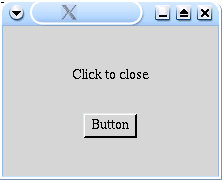
\includegraphics[width=2.3126in,height=1.8752in]{ub-img/ub-img50.jpg}
\end{center}

{\sffamily\bfseries Figure 18-1:}
{\sffamily TestDialog window}

\bigskip

This example program begins by
declaring a class, \texttt{TestDialog}. The line

\iconcode{
\>   class TestDialog : Dialog()}

\noindent
indicates that \texttt{TestDialog} is a \index{subclass}subclass of the
class \texttt{Dialog} that is defined in the toolkit. This subclass
relationship is true of all dialog windows. 

The remainder of the class's code is contained in a single method,
\texttt{component\_setup().} This method is invoked by the toolkit; it
is a convenient place to setup the dialog's content.
Inside the \texttt{component\_setup()} method is the code that adds
the label to the dialog:

\iconcode{
\>   l := Label("label=Click to
close","pos=50\%,33\%",
"align=c,c") \\
\>   add(l)}

\noindent This assigns \texttt{l} to a new \texttt{Label} object
and sets the label string. The horizontal position is set to 50 percent of
the window width and the vertical to 33 percent of the window height.
The alignment of the object is centered both vertically and
horizontally about the position. Finally, the label is added to the
dialog with the line \texttt{add(l)}.

The code to add a button is very similar, but a \texttt{TextButton}
object is created rather than a \texttt{Label} object, and the vertical
position is 66 percent of the window height. 

The next line is more interesting:

\iconcode{
\>   b.connect(self, "dispose", ACTION\_EVENT)
}

\noindent This adds a \textit{listener} to the button, and tells the toolkit
than whenever the button fires an \ \texttt{ACTION\_EVENT}, which it will
when it is pressed, the \texttt{dispose()} method in the class
\texttt{self}, should be invoked. \ \texttt{self} of course refers to
the \texttt{TestDialog} class, and \texttt{dispose()} is a method
inherited from the base class \texttt{Dialog}, which simply closes the
window. \ So all this means is that when the button is pressed, the
dialog will close.

The next line sets the attributes of the dialog window, including its
initial size. Try changing these values to experiment with other dialog
styles.

\iconcode{
\>   attrib("size=215,150",
"bg=light gray",
"font=serif",
"resize=on")}

After the class comes a standard Icon \texttt{main()} procedure. This
simply creates an instance of the dialog and invokes the method
\texttt{show\_modal()}.
This call displays the dialog window and goes into the
toolkit's event handling loop. 

\section{Positioning Objects}

The button and label were positioned above using
percentages of the window size. An object can also be
positioned by giving an absolute position, or by giving a percentage
plus or minus an offset. So the following are all valid position
specifiers:

\iconcode{
\>   \ \ "100" \\
\>   \ \ "10\%" \\
\>   \ \ "25\%+10" \\
\>   \ \ "33\%-10"
}

Positions are often specified in \index{constructor}constructors
with \texttt{x} and \texttt{y} values separated by commas. By default,
positions are relative to the top left corner of the object.
The \texttt{"align"}
attribute, which takes two alignment specifiers, changes this
default. The first alignment specifier is an
\texttt{"l"},
\texttt{"c"}\texttt{,} or
\texttt{"r"}, for left, center, or right
horizontal alignment, respectively; the second is a
\texttt{"t"},
\texttt{"c"}, or
\texttt{"b"}, for top, center, or bottom
vertical alignment, respectively. Another attribute,
\texttt{"size"}, has specifiers that take the
same format as the position attribute. Most of the toolkit objects
default to sensible sizes, and the size attribute can often be omitted.
For example, a button's size defaults fit its string label
based on the font in use.

The method \texttt{attrib(attribs...)} in utility class
\texttt{SetFields} implements \index{attribute!GUI widget}attribute
processing, mostly farming out work to special-purpose methods
that can be called directly: \texttt{set\_pos(x,y)},
\texttt{set\_label(s)}, \texttt{set\_align(horizontal, vertical)}, and
\texttt{set\_size(w, }\texttt{h)}. Other than these setter methods,
Icon graphics attributes can be interspersed. \ For example, the
attribute \texttt{"bg=green"} will set the
object's background color.

Here are some examples of position, alignment, and size parameters, and
a description of their meaning. In the call

\iconcode{
\>   attrib("pos=50\%,100",
"align=c,t",
"size=80\%,200")
}

\noindent
the object is centered horizontally in the window, using 80
percent of the width; vertically its top starts at 100 and its
height is 200 pixels. In contrast, the code

\iconcode{
\>   attrib("pos=100\%,100\%",
"align=r,b",
"size=50\%,50\%")
}

\noindent
specifies that the object fills up the bottom right quarter of the
window. The call

\iconcode{
\>   attrib("pos=33\%+20,0\%",
"size=100,100\%")
}

\noindent
directs that the object's left hand side is at
one-third of the window size plus 20 pixels; it is 100 pixels wide. It
fills the whole window vertically.

\section{A More Complex Dialog Example}

Now it's time to introduce some more component types.
Listing 18-2 shows our next example program in full.

\bigskip

{\sffamily\bfseries
Listing 18-2}

{\sffamily\bfseries
SecondTest Program}

\iconcode{
import gui \\
\$include "guih.icn" \\

class SecondTest : Dialog( \\
\>   \# Class variables representing objects in the dialog. \\
\>   text\_list, table, list, text\_field, \\
\>    \\
\>   
\>   oses, languages, shares \ \ \ \ \# Some data variables. \\
\>   ) \\
\ \\
\>   \# \\
\>   \# Add a line to the end of the text list \\
\>   \# \\
\>   method put\_line(s) \\
\>   \ \ \ local l := text\_list.get\_contents() \\
\>   \ \ \ put(l, s) \\
\>   \ \ \ text\_list.set\_contents(l) \\
\>   \ \ \ text\_list.goto\_pos(*l) \\
\>   end \\
\ \\
\>   \# \\
\>   \# Event handlers - produce a line of interest. \\
\>   \# \\
\>   method handle\_check\_box\_1(ev) \\
\>   \ \ \ put\_line("Favorite OS is "
{\textbar}{\textbar} oses[1]) \\
\>   end \\
\>   method handle\_check\_box\_2(ev) \\
\>   \ \ \ put\_line("Favorite OS is "
{\textbar}{\textbar} oses[2]) \\
\>   end \\
\>   method handle\_check\_box\_3(ev) \\
\>   \ \ \ put\_line("Favorite OS is "
{\textbar}{\textbar} oses[3]) \\
\>   end \\
\>   method handle\_text\_field(ev) \\
\>   \ \ \ put\_line("Contents = "
{\textbar}{\textbar} text\_field.get\_contents()) \\
\>   end \\
\>   method handle\_list(ev) \\
\>   \ \ \ put\_line("Favorite language is
" {\textbar}{\textbar} languages[list.get\_selection()]) \\
\>   end \\
\>   method handle\_text\_menu\_item\_2(ev) \\
\>   \ \ \ put\_line("You selected the menu
item") \\
\>   end \\
\ \\
\>   \# \\
\>   \# The quit menu item \\
\>   \# \\
\>   method handle\_quit(ev) \\
\>   \ \ \ dispose() \\
\>   end \\
\ \\
\>   method handle\_table(ev) \\
\>   \ \ \ local i := table.get\_selections()[1] \\
\>   \ \ \ put\_line(shares[i][1] {\textbar}{\textbar} "
is trading at " {\textbar}{\textbar} shares[i][2]) \\
\>   end \\
\ \\
\>   method handle\_table\_column\_1(ev) \\
\>   \ \ \ put\_line("Clicked on column
1") \\
\>   end \\
\ \\
\>   method handle\_table\_column\_2(ev) \\
\>   \ \ \ put\_line("Clicked on column
2") \\
\>   end
\ \\
\>   \# \\
\>   \# This method is invoked for a component which may potentially want \\
\>   \# to handle an event (by firing an event to its listeners for\\
\>   \# example). \ A dialog is just another custom component, and so it can\\
\>   \# override this method to do any custom processing. \\
\>   \# \\
\>   method handle\_event(ev) \\
\>   \ \ \ put\_line("Icon event "
{\textbar}{\textbar} ev) \\
\>   \ \ \ self.Dialog.handle\_event(ev) \\
\>   end \\
\ \\
\>   method component\_setup() \\
\>   \ \ \ local menu\_bar, menu, panel\_1, panel\_2, panel\_3, panel\_4, panel\_5, \\
\>   \ \ \ \ \ \ \ \ \ label\_1, label\_2, label\_3, label\_4, label\_5, \\
\>   \ \ \ \ \ \ \ \ \ quit\_menu\_item, text\_menu\_item\_2, \\
\>   \ \ \ \ \ \ \ \ \ check\_box\_1, check\_box\_2, check\_box\_3, \\
\>   \ \ \ \ \ \ \ \ \ table\_column\_1, table\_column\_2, check\_box\_group \\
\ \\
\>   \ \ \ \# \\
\>   \ \ \ \# Initialize some data for the objects. \\
\>   \ \ \ \# \\
\>   \ \ \ oses := ["Windows",
"Linux",
"Solaris"] \\
\>   \ \ \ languages := ["C",
"C++", "Java",
"Icon"] \\
\>   \ \ \ shares := [["Microsoft",
"101.84"],
["Oracle",
"32.52"],
["IBM",
"13.22"], \\
\>\>\>
["Intel",
"142.00"]] \\
\ \\
\>   \ \ \ \# \\
\>   \ \ \ \# Set the attributes, then setup a simple menu system \\
\>   \ \ \ \# \\
\>   \ \ \ attrib("size=490,400",
"min\_size=490,400",
"font=sans", \\
\>   \ \ \ \ \ \ \ \ \ \ "bg=light
gray","label=Second example",
"resize=on") \\
\>   \ \ \ menu\_bar := MenuBar() \\
\>   \ \ \ menu := Menu("label=File") \\
\>   \ \ \ quit\_menu\_item := TextMenuItem("label=Quit") \\
\>   \ \ \ quit\_menu\_item.connect(self, "handle\_quit", ACTION\_EVENT) \\
\>   \ \ \ menu.add(quit\_menu\_item) \\
\>   \ \ \ text\_menu\_item\_2 :=
TextMenuItem("label=Message") \\
\>   \ \ \ text\_menu\_item\_2.connect(self,
"handle\_text\_menu\_item\_2",\\
\>\>\>\>\>ACTION\_EVENT) \\
\>   \ \ \ menu.add(text\_menu\_item\_2) \\
\>   \ \ \ menu\_bar.add(menu) \\
\>   \ \ \ add(menu\_bar) \\
\ \\
\>   \ \ \ \# \\
\>   \ \ \ \# Set-up the checkbox panel \\
\>   \ \ \ \# \\
\>   \ \ \ check\_box\_group := CheckBoxGroup() \\
\>   \ \ \ panel\_1 := Panel("pos=20,50",
"size=130,130") \\
\>   \ \ \ label\_2 := Label("pos=0,0",
"internal\_alignment=l",
"label=Favorite OS") \\
\>   \ \ \ panel\_1.add(label\_2) \\
\>   \ \ \ check\_box\_1 :=
CheckBox("pos=0,30") \\
\>   \ \ \ check\_box\_1.set\_label(oses[1]) \\
\>   \ \ \ check\_box\_1.connect(self,
"handle\_check\_box\_1", ACTION\_EVENT) \\
\>   \ \ \ check\_box\_group.add(check\_box\_1) \\
\>   \ \ \ panel\_1.add(check\_box\_1) \\
\>   \ \ \ check\_box\_2 :=
CheckBox("pos=0,60") \\
\>   \ \ \ check\_box\_2.set\_label(oses[2]) \\
\>   \ \ \ check\_box\_group.add(check\_box\_2) \\
\>   \ \ \ check\_box\_2.connect(self,
"handle\_check\_box\_2", ACTION\_EVENT) \\
\>   \ \ \ panel\_1.add(check\_box\_2) \\
\>   \ \ \ check\_box\_3 :=
CheckBox("pos=0,90") \\
\>   \ \ \ check\_box\_3.set\_label(oses[3]) \\
\>   \ \ \ check\_box\_group.add(check\_box\_3) \\
\>   \ \ \ check\_box\_3.connect(self,
"handle\_check\_box\_3", ACTION\_EVENT) \\
\>   \ \ \ panel\_1.add(check\_box\_3) \\
\>   \ \ \ add(panel\_1) \\
\>   \ \ \ \# \\
\>   \ \ \ \# The text-list of messages. \\
\>   \ \ \ \# \\
\>   \ \ \ panel\_2 := Panel("pos=220,50",
"size=100\%-240,50\%-60") \\
\>   \ \ \ label\_1 := Label("pos=0,0",
"internal\_alignment=l",
"label=Messages") \\
\>   \ \ \ panel\_2.add(label\_1) \\
\>   \ \ \ text\_list :=
TextDisplay("pos=0,30",
"size=100\%,100\%-30") \\
\>   \ \ \ text\_list.set\_contents([]) \\
\>   \ \ \ panel\_2.add(text\_list) \\
\>   \ \ \ add(panel\_2) \\
\>   \ \ \ \# \\
\>   \ \ \ \# The table of shares. \\
\>   \ \ \ \# \\
\>   \ \ \ panel\_3 :=
Panel("pos=220,50\%","size=100\%-240,50\%-40") \\
\>   \ \ \ table :=
Table("pos=0,30","size=100\%,100\%-30",
"select\_one") \\
\>   \ \ \ table.connect(self,
"handle\_table",
SELECTION\_CHANGED\_EVENT) \\
\>   \ \ \ table.set\_contents(shares) \\
\ \\
\>   \ \ \ table\_column\_1 :=
TableColumn("label=Company",
"internal\_alignment=l", \\
\>   \ \ \ \ \ \ \ \ \ \ \ \ \ \ \ \ \ \ \ \ \ \ \ \ \ \ \ \ \ \ \ \ \ "column\_width=100") \\
\>   \ \ \ table\_column\_1.connect(self,
"handle\_table\_column\_1", ACTION\_EVENT) \\
\>   \ \ \ table.add\_column(table\_column\_1) \\
\>   \ \ \ table\_column\_2 := TableColumn("label=Share
price",
"internal\_alignment=r", \\
\>   \ \ \ \ \ \ \ \ \ \ \ \ \ \ \ \ \ \ \ \ \ \ \ \ \ \ \ \ \ \ \ \ \ "column\_width=100") \\
\>   \ \ \ table\_column\_2.connect(self,
"handle\_table\_column\_2", ACTION\_EVENT) \\
\>   \ \ \ table.add\_column(table\_column\_2) \\
\>   \ \ \ panel\_3.add(table) \\
\>   \ \ \ label\_5 := Label("pos=0,0",
"internal\_alignment=l",
"label=Shares") \\
\>   \ \ \ panel\_3.add(label\_5) \\
\>   \ \ \ add(panel\_3) \\
\>   \ \ \ \# \\
\>   \ \ \ \# The drop-down list of languages. \\
\>   \ \ \ \# \\
\>   \ \ \ panel\_4 := Panel("pos=20,190",
"size=180,50") \\
\>   \ \ \ list := List("pos=0,30", "size=100,") \\
\>   \ \ \ list.connect(self,
"handle\_list", SELECTION\_CHANGED\_EVENT) \\
\>   \ \ \ list.set\_selection\_list(languages) \\
\>   \ \ \ panel\_4.add(list) \\
\>   \ \ \ label\_3 := Label("pos=0,0", "internal\_alignment=l",
"label=Favorite language") \\
\>   \ \ \ panel\_4.add(label\_3) \\
\>   \ \ \ add(panel\_4) \\
\>   \ \ \ \# \\
\>   \ \ \ \# The text field. \\
\>   \ \ \ \# \\
\>   \ \ \ panel\_5 := Panel("pos=20,280",
"size=180,50") \\
\>   \ \ \ label\_4 := Label("pos=0,0",
"internal\_alignment=l",
"label=Enter a string") \\
\>   \ \ \ panel\_5.add(label\_4) \\
\>   \ \ \ text\_field :=
TextField("pos=0,30",
"size=130,",
"draw\_border=t") \\
\>   \ \ \ text\_field.connect(self,
"handle\_text\_field",
TEXTFIELD\_CHANGED\_EVENT) \\
\>   \ \ \ panel\_5.add(text\_field) \\
\>   \ \ \ add(panel\_5) \\
\>   end \\
end \\
\# \\
\# Simple main procedure just creates the dialog. \\
\# \\
procedure main() \\
\>   SecondTest().show\_modal() \\
end
}


\begin{center}
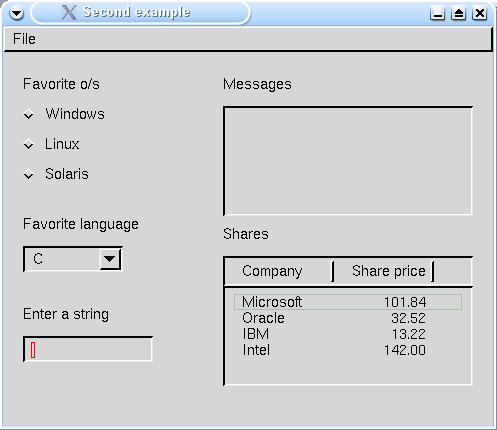
\includegraphics[width=4.0756in,height=3.6465in]{ub-img/ub-img51.jpg}
\end{center}

{\sffamily\bfseries Figure 18-2:}
{\sffamily SecondTest window}

\bigskip

Start examining this program with the \texttt{component\_setup()}
method at the end. This method initializes some data and
sets attributes. This includes several Icon graphics attributes,
as well as the minimum size, which is an attribute of the
\texttt{Dialog} class.

The next part creates a \index{menu bar}menu bar structure.
Menu structures are presented in detail later in this chapter, but for
now observe that this code creates two textual menu items within a
\texttt{Menu} object, which is itself within a \texttt{MenuBar} object,
which is added to the dialog. \ Both menu items are connected to event
handler methods.

The next section sets up three \index{check boxes}check boxes,
placed together with the label "Favorite OS" in a \texttt{Panel} object,
which serves as a container for other objects that logically are treated
as a whole. Objects within a \texttt{Panel} have their size and
position computed relative
to the \texttt{Panel} rather than the window. So, for example, the
first \texttt{Label} object is positioned with
\texttt{"pos=0,0"}. This places it at the
top left-hand corner of the \texttt{Panel}, not the top left of the
window. Percentage specifications similarly relate to the enclosing
\texttt{Panel}.

Each \texttt{CheckBox} is a separate object. To make the three check
boxes behave as a group so that when one is checked
another is unchecked, they are placed in a
\texttt{CheckBoxGroup} object; this just
``brackets'' them together. When grouped
together in this way the checkboxes are called \index{radio
buttons}\textit{radio buttons} because they work like the
tuner buttons found on old car radios. Note that each
\texttt{CheckBox} is added to the \texttt{CheckBoxGroup} \textit{and}
the \texttt{Panel}.

The next section is a \texttt{Panel} that holds a label
("Messages") and a \texttt{TextList}
object. In this case the object holds a list of message
strings that scroll by like a terminal window. A \texttt{TextList}
object can also be used for selecting one or more items from a list of
strings and there is an \texttt{EditableTextList},
which can be used for editing text.

The third panel contains a label ("Shares"),
and a \texttt{Table} object, which is used for displaying tabular data.
Note that class \texttt{Table} has nothing to do with
Icon's table data type. Adding a \texttt{TableColumn}
object to the table sets up each column. A table column's
initial column width is specified with attribute \texttt{column\_width}
and the alignment of the column's contents is set with
attribute \texttt{internal\_alignment}. Attribute
\texttt{select\_one} configures the table to allow one row to
be highlighted at a time. The default is not to allow highlighting of
rows; the other option is to allow several to be highlighted at once
with \texttt{select\_many}.

The next panel contains another label ("Favorite
language") and a drop-down list of selections, created
using the \texttt{List} class. The selections are set using the
\texttt{set\_selection\_list()} method. The final panel contains a
label ("Enter a string") and a
\texttt{TextField} object, which is used to obtain entry of a string
from the \index{keyboard}keyboard.

Several of the components are connected to event handlers in the class.
Each handler method adds a line to the list of strings in the
\texttt{TextList} by calling the \texttt{put\_line()} method. The text
list thus gives an idea of the events being produced by the toolkit.
The exception is the menu item \texttt{Quit}, which exits the
program.

This dialog overrides the \texttt{handle\_event()} method that is
invoked by the toolkit for any component (including dialogs)
that may elect to handle an event. In this case, the dialog just
prints out the Icon event code for the particular event. This method
also checks for the Alt-q keyboard combination, which closes the
dialog.

\section{More About Event Handling}

As shown above, components generate events when
something of interest happens. For example, a button generates an
\texttt{ACTION\_EVENT} when it is pressed. Different components
generate different events, but there are some basic events generated by
all components:

\vspace{0.15in}
\begin{xtabular}{m{2.2in} m{3.5in}}
\texttt{MOUSE\_PRESS\_EVENT} &
 a mouse press within the component's
region.\\
\texttt{MOUSE\_DRAG\_EVENT} &
 a mouse drag within the component's
region.\\
\texttt{MOUSE\_RELEASE\_EVENT} &
 a mouse release within the component's
region.\\
\end{xtabular}
\vspace{0.15in}

\noindent For any non-mouse events, the \texttt{Dialog} class fires an
\texttt{ICON\_EVENT}.

Event are passed to listeners in an \texttt{Event}
object. This object contains three fields,
with corresponding getter methods, as follows:

\vspace{0.15in}
\begin{xtabular}{m{1.2in} m{4.7in}}
\texttt{get\_source()} & Returns the component which fired the event.\\
\texttt{get\_type()} & Returns the type code, eg \texttt{ICON\_EVENT}\\
\texttt{get\_param()} &
Returns an arbitrary parameter depending on the type. In
nearly all cases this is the original underlying Icon graphics event.\\
\end{xtabular}
\vspace{0.15in}

The \texttt{get\_param()} method is necessary, for example, to
distinguish between a left mouse click and a right mouse click on a
\texttt{MOUSE\_RELEASE\_EVENT}; for instance 

\iconcode{
\>   method on\_release(ev) \\
\>   \ \ \ if ev.get\_param() === \&rrelease then \\
\>   \ \ \ \ \ \ ... process right mouse up \\
\>   end
}

\section{Containers}

\textit{Containers} are components that contain other components.
The \texttt{Dialog} class is a container, as is
the \texttt{Panel} class seen in the last example.
Two other useful \index{container,
GUI class}container objects in the standard toolkit are \texttt{TabSet}
and \texttt{OverlaySet}.

\subsection*{\texttt{TabSet}}

This class contains several \index{tab,GUI class}tabbed panes, any one of which
is displayed at any given time. The user switches between panes by clicking on
labeled tabs at the top of the object. The \texttt{TabSet} contains several
\texttt{TabItems}, each of which contains the components for that particular
pane. To illustrate this, Listing 18-3 presents a simple example of a
\texttt{TabSet} that contains three \texttt{TabItems}, each of which contains a
single label.

\bigskip

{\sffamily\bfseries
Listing 18-3

TabSet Program}

\iconcode{
import gui \\
\$include "guih.icn" \\
\# \\
\# Simple example of a TabSet \\
\# \\
class Tabs : Dialog(quit\_button) \\
\>   method change(e) \\
\>   \ \ \ write("The tabset selection
changed") \\
\>   end \\
\ \\
\>   method component\_setup() \\
\>   \ \ \ local tab\_set, tab\_item\_1, tab\_item\_2, tab\_item\_3 \\
\>   \ \ \ attrib("size=355,295", "font=sans", "bg=light gray", \\
\>\>\> "label=TabSet example", "resize=on") \\
\>   \ \ \ \#  \\
\>   \ \ \ \# Create the TabSet \\
\>   \ \ \ tab\_set := TabSet("pos=20,20",
"size=100\%-40,100\%-80") \\
\>   \ \ \ \#  \\
\>   \ \ \ \# First, second, and third panes \\
\>   \ \ \ \# \\
\>   \ \ \ tab\_item\_1 := TabItem("label=Pane 1") \\
\>   \ \ \ tab\_item\_1.add(Label("pos=50\%,50\%", "align=c,c",
                            "label=Label 1")) \\
\>   \ \ \ tab\_set.add(tab\_item\_1) \\
\>   \ \ \ tab\_item\_2 := TabItem("label=Pane 2") \\
\>   \ \ \ tab\_item\_2.add(Label("pos=50\%,50\%",
                                  "align=c,c", "label=Label 2")) \\
\>   \ \ \ tab\_set.add(tab\_item\_2) \\
\>   \ \ \ tab\_item\_3 := TabItem("label=Pane 3") \\
\>   \ \ \ tab\_item\_3.add(Label("pos=50\%,50\%",
"align=c,c", "label=Label 3")) \\
\>   \ \ \ tab\_set.add(tab\_item\_3) \\
\>   \ \ \ tab\_set.set\_which\_one(tab\_item\_1) \\
\>   \ \ \ tab\_set.connect(self, "change",
SELECTION\_CHANGED\_EVENT) \\
\>   \ \ \ add(tab\_set) \\
\>   \ \ \ \# \\
\>   \ \ \ \# Add a quit button; close the dialog when it is pressed \\
\>   \ \ \ quit\_button :=
TextButton("pos=50\%,100\%-30", "align=c,c", "label=Quit") \\
\>   \ \ \ quit\_button.connect(self,
"dispose", ACTION\_EVENT) \\
\>   \ \ \ add(quit\_button) \\
\>   \ \ \ connect(self, "dispose",
CLOSE\_BUTTON\_EVENT) \\
\>   end \\
end \\
procedure main() \\
\>   Tabs().show\_modal() \\
end
}


The resulting window is shown in Figure 18-3:

\begin{center}
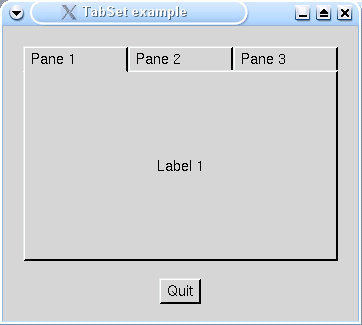
\includegraphics[width=3.1272in,height=2.7299in]{ub-img/ub-img52.jpg}
\linebreak
{\sffamily\bfseries Figure 18-3:}
{\sffamily TabSet example window}
\end{center}

\bigskip

\noindent One interesting point in this dialog is the line:

\iconcode{
\>   connect(self, "dispose", CLOSE\_BUTTON\_EVENT)}


\noindent A dialog generates an event whenever the close button is
pressed. Connecting this event to the \texttt{dispose}
method configures the dialog to close when this button is
pressed.

\subsection*{\texttt{OverlaySet}}

\index{overlay, GUI class}An \texttt{OverlaySet} is like a \texttt{TabSet},
but the pane on display is under program control; there are no
tabs to click. Instead of adding items to \texttt{TabItem} structures,
\texttt{OverlayItem} objects are used. An empty \texttt{OverlayItem} can be
used when the area should be blank. The current \texttt{OverlayItem} on
display is set by \texttt{set\_which\_one(x)}, where \texttt{x} is
the desired \texttt{OverlayItem}.

\section{Menu Structures}

The toolkit provides the standard building blocks required to create
a \index{menu}menu system (see Table 18-1). Customized components can
be added; this is discussed later.

\begin{center}
{\centering\sffamily\bfseries
Table 18-1 \\
Standard Menu System Components}
\end{center}
\begin{flushleft}
\begin{xtabular}{|m{1.6in}|m{4.3in}|}
\hline
\sffamily\bfseries Component &
\sffamily\bfseries Description\\\hline
\texttt{MenuBar} &
The menu area along the top of the window, containing one or
more \texttt{Menu}s.\\\hline
\texttt{MenuButton} &
A floating menu bar containing one \texttt{Menu}.\\\hline
\texttt{Menu} &
A drop down menu pane containing other \texttt{Menu}s or menu
components.\\\hline
\texttt{TextMenuItem} &
A textual menu item.\\\hline
\ttfamily \texttt{CheckBoxMenuItem}  &
A checkbox in a menu which can be part of a \texttt{CheckBoxGroup} if
desired.\\\hline
\texttt{MenuSeparator} &
A vertical separation line between items.\\\hline
\end{xtabular}
\end{flushleft}
Items in a \texttt{Menu} can have left and right labels as well as
customized left and right images. To see how this all fits together,
Listing 18-4 shows our next example program.

\bigskip

{\sffamily\bfseries
Listing 18-4}

{\sffamily\bfseries
A Menu Example Program}

\iconcode{
import gui \\
\$include "guih.icn" \\
\ \\
class MenuDemo : Dialog() \\
\>   method component\_setup() \\
\>\>    local file\_menu, menu\_bar, check\_box\_group, text\_menu\_item, \\
\>\>\>   labels\_menu, images\_menu, checkboxes\_menu, group\_menu, \\
\>\>\>   alone\_menu, menu\_button, check\_box\_menu\_item, button\_menu \\
\ \\
\>\>   attrib("size=426,270", "font=sans", "bg=light gray",
              "label=Menu example") \\
\>   \ \ \ check\_box\_group := CheckBoxGroup() \\
\ \\
\>   \ \ \ \# \\
\>   \ \ \ \# Create the menu bar. The position and size default to \\
\>   \ \ \ \# give a bar covering the top of the window. \\
\>   \ \ \ \# The first menu ("File") - just contains one text item. \\
\>   \ \ \ menu\_bar := MenuBar() \\
\>   \ \ \ file\_menu := Menu("label=File") \\
\>   \ \ \ text\_menu\_item := TextMenuItem("label=Quit") \\
\>   \ \ \ text\_menu\_item.connect(self, "dispose", ACTION\_EVENT) \\
\>   \ \ \ file\_menu.add(text\_menu\_item) \\
\>   \ \ \ menu\_bar.add(file\_menu) \\
\ \\
\>   \ \ \ \# \\
\>   \ \ \ \# The second menu ("Labels") - add some labels, followed by \\
\>   \ \ \ \# a separator and another text item \\
\>   \ \ \ labels\_menu := Menu("label=Labels") \\
\>   \ \ \ labels\_menu.add(TextMenuItem("label=One")) \\
\>   \ \ \ labels\_menu.add(TextMenuItem("label=Two", "label\_left=ABC")) \\
\>   \ \ \ labels\_menu.add(MenuSeparator()) \\
\>   \ \ \ labels\_menu.add(TextMenuItem("label=Three", "label\_right=123")) \\
\>   \ \ \ \# \\
\>   \ \ \ \# A sub-menu in this menu, labeled "Images", contains \\
\>   \ \ \ \# three text items with custom images. The rather unwieldy \\
\>   \ \ \ \# strings create a triangle, a circle and a rectangle. \\
\>   \ \ \ images\_menu := Menu("label=Images") \\
\>   \ \ \ text\_menu\_item := TextMenuItem("label=One") \\
\>   \ \ \ text\_menu\_item.set\_img\_left("15,c1,\~{}\~{}\~{}\~{}\~{}\~{}\~{}0\~{}\~{}\~{}\~{}\~{}\~{}\~{}\_ \\
\>\>\~{}\~{}\~{}\~{}\~{}\~{}\~{}0\~{}\~{}\~{}\~{}\~{}\~{}\~{}\~{}\~{}\~{}\~{}\~{}\~{}000\~{}\~{}\~{}\~{}\~{}\~{}\~{}\~{}\~{}\~{}\~{}\~{}000\~{}\~{}\~{}\~{}\~{}\~{}\_ \\
\>\>\~{}\~{}\~{}\~{}\~{}00\~{}00\~{}\~{}\~{}\~{}\~{}\~{}\~{}\~{}\~{}\~{}00\~{}00\~{}\~{}\~{}\~{}\~{}\~{}\~{}\~{}\~{}00\~{}\~{}\~{}00\~{}\~{}\~{}\~{}\_ \\
\>\>\~{}\~{}\~{}\~{}00\~{}\~{}\~{}00\~{}\~{}\~{}\~{}\~{}\~{}\~{}00\~{}\~{}\~{}\~{}\~{}00\~{}\~{}\~{}\~{}\~{}\~{}00\~{}\~{}\~{}\~{}\~{}00\~{}\~{}\~{}\_ \\
\>\>\~{}\~{}00\~{}\~{}\~{}\~{}\~{}\~{}\~{}00\~{}\~{}\~{}\~{}00\~{}\~{}\~{}\~{}\~{}\~{}\~{}00\~{}\~{}\~{}00\~{}\~{}\~{}\~{}\~{}\~{}\~{}\~{}\~{}00\~{}\_ \\
\>\>\~{}0000000000000\~{}000000000000000") \\
\>   \ \ \ images\_menu.add(text\_menu\_item) \\
\>   \ \ \ text\_menu\_item :=
TextMenuItem("label=Two") \\
\>   \ \ \ text\_menu\_item.set\_img\_left("15,c1,\~{}\~{}\~{}\~{}\~{}\~{}000\~{}\~{}\~{}\~{}\~{}\~{}\_ \\
\>\>\~{}\~{}\~{}\~{}0000000\~{}\~{}\~{}\~{}\~{}\~{}000\~{}\~{}\~{}\~{}\~{}000\~{}\~{}\~{}\~{}00\~{}\~{}\~{}\~{}\~{}\~{}\~{}00\~{}\~{}\_ \\
\>\>\~{}00\~{}\~{}\~{}\~{}\~{}\~{}\~{}\~{}\~{}00\~{}\~{}0\~{}\~{}\~{}\~{}\~{}\~{}\~{}\~{}\~{}\~{}\~{}0\~{}00\~{}\~{}\~{}\~{}\~{}\~{}\~{}\~{}\~{}\~{}\~{}00\_ \\
\>\>00\~{}\~{}\~{}\~{}\~{}\~{}\~{}\~{}\~{}\~{}\~{}0000\~{}\~{}\~{}\~{}\~{}\~{}\~{}\~{}\~{}\~{}\~{}00\~{}0\~{}\~{}\~{}\~{}\~{}\~{}\~{}\~{}\~{}\~{}\~{}0\~{}\_ \\
\>\>\~{}00\~{}\~{}\~{}\~{}\~{}\~{}\~{}\~{}\~{}00\~{}\~{}\~{}00\~{}\~{}\~{}\~{}\~{}\~{}\~{}00\~{}\~{}\~{}\~{}000\~{}\~{}\~{}\~{}\~{}000\~{}\~{}\_ \\
\>\>\~{}\~{}\~{}\~{}0000000\~{}\~{}\~{}\~{}\~{}\~{}\~{}\~{}\~{}\~{}000\~{}\~{}\~{}\~{}\~{}\~{}") \\
\>   \ \ \ images\_menu.add(text\_menu\_item) \\
\>   \ \ \ text\_menu\_item :=
TextMenuItem("label=Three") \\
\>   \ \ \ text\_menu\_item.set\_img\_left("15,c1,\_ \\
\>\>000000000000000000000000000000\_ \\
\>\>00\~{}\~{}\~{}\~{}\~{}\~{}\~{}\~{}\~{}\~{}\~{}0000\~{}\~{}\~{}\~{}\~{}\~{}\~{}\~{}\~{}\~{}\~{}0000\~{}\~{}\~{}\~{}\~{}\~{}\~{}\~{}\~{}\~{}\~{}00\_ \\
\>\>00\~{}\~{}\~{}\~{}\~{}\~{}\~{}\~{}\~{}\~{}\~{}0000\~{}\~{}\~{}\~{}\~{}\~{}\~{}\~{}\~{}\~{}\~{}0000\~{}\~{}\~{}\~{}\~{}\~{}\~{}\~{}\~{}\~{}\~{}00\_ \\
\>\>00\~{}\~{}\~{}\~{}\~{}\~{}\~{}\~{}\~{}\~{}\~{}0000\~{}\~{}\~{}\~{}\~{}\~{}\~{}\~{}\~{}\~{}\~{}0000\~{}\~{}\~{}\~{}\~{}\~{}\~{}\~{}\~{}\~{}\~{}00\_ \\
\>\>00\~{}\~{}\~{}\~{}\~{}\~{}\~{}\~{}\~{}\~{}\~{}0000\~{}\~{}\~{}\~{}\~{}\~{}\~{}\~{}\~{}\~{}\~{}00\_ \\
\>\>000000000000000000000000000000") \\
\>   \ \ \ images\_menu.add(text\_menu\_item) \\
\>   \ \ \ labels\_menu.add(images\_menu) \\
\>   \ \ \ menu\_bar.add(labels\_menu) \\
\ \\
\>   \ \ \ \# \\
\>   \ \ \ \# The third menu
("Checkboxes") \\
\>   \ \ \ \# Sub-menu - "Group" - two
checkboxes in a checkbox group. \\
\>   \ \ \ \# \\
\>   \ \ \ checkboxes\_menu :=
Menu("label=Checkboxes") \\
\>   \ \ \ group\_menu :=
Menu("label=Group") \\
\>   \ \ \ check\_box\_menu\_item :=
CheckBoxMenuItem("label=One") \\
\>   \ \ \ check\_box\_group.add(check\_box\_menu\_item) \\
\>   \ \ \ group\_menu.add(check\_box\_menu\_item) \\
\>   \ \ \ check\_box\_menu\_item :=
CheckBoxMenuItem("label=Two") \\
\>   \ \ \ check\_box\_group.add(check\_box\_menu\_item) \\
\>   \ \ \ group\_menu.add(check\_box\_menu\_item) \\
\>   \ \ \ checkboxes\_menu.add(group\_menu) \\
\>   \ \ \ \# \\
\>   \ \ \ \# Sub-menu - "Alone" - two
checkboxes on their own \\
\>   \ \ \ \# \\
\>   \ \ \ alone\_menu := Menu() \\
\>   \ \ \ alone\_menu.set\_label("Alone") \\
\>   \ \ \ check\_box\_menu\_item\_3 :=
CheckBoxMenuItem("label=Three") \\
\>   \ \ \ alone\_menu.add(check\_box\_menu\_item\_3) \\
\>   \ \ \ check\_box\_menu\_item\_4 :=
CheckBoxMenuItem("label=Four") \\
\>   \ \ \ alone\_menu.add(check\_box\_menu\_item\_4) \\
\>   \ \ \ checkboxes\_menu.add(alone\_menu) \\
\>   \ \ \ menu\_bar.add(checkboxes\_menu) \\
\>   \ \ \ add(menu\_bar) \\
\>   \ \ \ \# \\
\>   \ \ \ \# Finally, create a menu button - a mini floating menu with \\
\>   \ \ \ \# one menu inside it. \\
\>   \ \ \ \# \\
\>   \ \ \ menu\_button :=
MenuButton("pos=350,50\%",
"align=c,c") \\
\>   \ \ \ \# \\
\>   \ \ \ \# This is the menu, its label appears on the button. \ It just\\
\>   \ \ \ \# contains a couple of text items for illustration purposes. \\
\>   \ \ \ \# \\
\>   \ \ \ button\_menu :=
Menu("label=Click") \\
\>   \ \ \ button\_menu.add(TextMenuItem("label=One")) \\
\>   \ \ \ button\_menu.add(TextMenuItem("label=Two")) \\
\>   \ \ \ menu\_button.set\_menu(button\_menu) \\
\>   \ \ \ add(menu\_button) \\
\>   end \\
end \\
\ \\
procedure main() \\
\>   MenuDemo().show\_modal() \\
end
}

The output of this program with the middle menu and its submenu open
appears in Figure 18-4.\\

\begin{center}
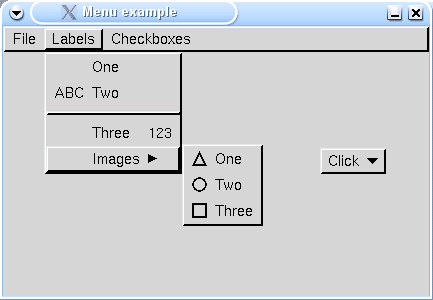
\includegraphics[width=4.2043in,height=2.7925in]{ub-img/ub-img53.jpg}
\end{center}

{\sffamily\bfseries Figure 18-4:}
{\sffamily Menus}

\section{Trees}

The toolkit contains a tree component, which can be used to represent
hierarchical data. \ To use it, it is necessary to create a tree-like
data structure of \texttt{Node} objects. Children are added to a
\texttt{Node} using its \texttt{add()} method. For example:

\iconcode{
root := Node("label=Root") \\
child1 := Node("label=Child1") \\
child2 := Node("label=Child2") \\
root.add(child1) \\
root.add(child2) \# ...etc
}

After setting up the tree of \texttt{Node}s, the root is passed
to the \texttt{Tree} for display:

\iconcode{
tree := Tree("pos=0,0",
"size=100,100")
tree.set\_root\_node(root)
}

\noindent The tree data structure can change dynamically over time. When this
occurs, the \texttt{Tree} must be notified of the change by invoking
the \texttt{tree\_structure\_changed()} method.

The \texttt{Tree} class generates events when the selected \texttt{Node}
(or \texttt{Node}s) changes, and also when part of the tree is expanded
or collapsed by the user.

The next example uses a \texttt{Tree} with a \texttt{Table} and a
\texttt{Sizer} to provide a file system explorer program.
The \texttt{Sizer} is a narrow area between
the tree and the table which can be dragged to resize both dynamically.
Because of the toolkit's relatively simple layout
mechanism, the resizing code in \texttt{handle\_sizer()} is quite
awkward.



\begin{center}
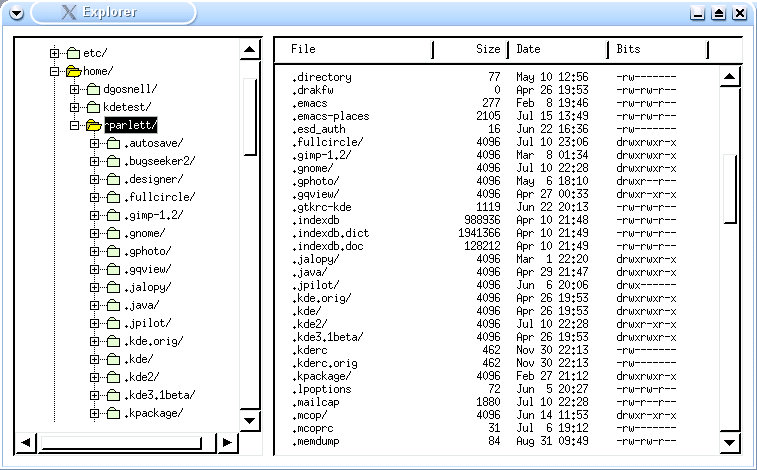
\includegraphics[width=5.8134in,height=3.4898in]{ub-img/ub-img54.jpg}
\end{center}

{\sffamily\bfseries Figure 18-5:}
{\sffamily Explorer}


\bigskip

{\sffamily\bfseries
Listing 18-5}

{\sffamily\bfseries
The Explorer Program}

\iconcode{
import gui \\
\ \\
\$include "keysyms.icn" \\
\$include "guih.icn" \\
\ \\
\# \\
\# A very simple filesystem explorer with a tree and a table. \\
\# \\
class Explorer : Dialog(tree, sizer, tbl) \\
\ \\
\>   \# \\
\>   \# Given a Node n, get the full file path it represents by \\
\>   \# traversing up the tree structure to the root. \\
\>   \# \\
\>   method get\_full\_path(n) \\
\>   \ \ \ local s := "" \\
\>   \ \ \ repeat \{ \\
\>   \ \ \ \ \ \ s := n.get\_label() {\textbar}{\textbar} s \\
\>   \ \ \ \ \ \ n := n.get\_parent\_node() {\textbar} break \\
\>   \ \ \ \ \ \ \} \\
\>   \ \ \ return s \\
\>   end \\
\ \\
\>   \# \\
\>   \# Invoked when a sub-tree is expanded (ie: the little + is \\
\>   \# clicked). \ An expansion event also includes contractions too \\
\>   \# \\
\>   method handle\_tree\_expansion() \\
\>   \ \ \ local n := tree.get\_last\_expanded() \\
\>   \ \ \ \# \\
\>   \ \ \ \# Check whether it was an expansion or a contraction. \ If \\
\>   \ \ \ \# an expansion, load the subtree and refresh the tree. \\
\>   \ \ \ \# \\
\>   \ \ \ if n.is\_expanded() then \{ \\
\>   \ \ \ \ \ \ load\_subtree(n) \\
\>   \ \ \ \ \ \ tree.tree\_structure\_changed() \\
\>   \ \ \ \ \ \ \} \\
\>   end \\
\ \\
\>   \# \\
\>   \# Invoked when a row in the tree is selected (or de-selected). \\
\>   \# If something is selected, load the table. We may not have something\\
\>   \# selected if the user contracted the parent node of the selected node. \\
\>   \# \\
\>   method handle\_tree\_selection() \\
\>   \ \ \ local n \\
\>   \ \ \ if n := tree.object\_get\_selections()[1] then \\
\>   \ \ \ \ \ \ load\_table(n) \\
\>   end \\
\ \\
\>   \# \\
\>   \# Given a Node n, load its children with the sub-directories. \\
\>   \# \\
\>   method load\_subtree(n) \\
\>   \ \ \ local name, r1, dir\_list := get\_directory\_list(get\_full\_path(n)) \\
\>   \ \ \ n.clear\_children() \\
\>   \ \ \ every name := !dir\_list[1] do \{ \\
\>   \ \ \ \ \ \ if (name \~{}== "./") \&
(name \~{}== "../") then \{ \\
\>   \ \ \ \ \ \ \ \ \ r1 :=
Node("always\_expandable=t") \\
\>   \ \ \ \ \ \ \ \ \ r1.set\_label(name) \\
\>   \ \ \ \ \ \ \ \ \ n.add(r1) \\
\>   \ \ \ \ \ \ \} \\
\>   \ \ \ \} \\
\>   end \\
\ \\
\>   \# \\
\>   \# Given a Node n, load the table with the sub-files and sub-directories.\\
\>   \# \\
\>   method load\_table(n) \\
\>   \ \ \ local s := get\_full\_path(n), l := [ ], t := get\_directory\_list(s) \\
\>   \ \ \ every el := !sort(t[1] {\textbar}{\textbar}{\textbar} t[2])
do \{ \\
\>   \ \ \ \ \ \ p := stat(s {\textbar}{\textbar} el) {\textbar}
stop("No stat") \\
\>   \ \ \ \ \ \ put(l, [el, p.size, ctime(p.mtime)[5:17], p.mode]) \\
\>   \ \ \ \ \ \ \} \\
\ \\
\>   \ \ \ tbl.set\_contents(l) \\
\>   \ \ \ tbl.goto\_pos(1, 0) \\
\>   end \\
\ \\
\>   \# \\
\>   \# The sizer has moved, so reset the sizes and positions of the \\
\>   \# table, tree and sizer. \ Then call resize() to reposition \\
\>   \# everything. \\
\>   \# \\
\>   method handle\_sizer(ev) \\
\>   \ \ \ result\_x := sizer.get\_curr\_pos() \\
\>   \ \ \ tree.set\_size(result\_x - 10, tree.h\_spec) \\
\>   \ \ \ sizer.set\_pos(result\_x, sizer.y\_spec) \\
\>   \ \ \ tbl.set\_pos(result\_x + 10, tbl.y\_spec) \\
\>   \ \ \ tbl.set\_size("100\%-" {\textbar}{\textbar} string(result\_x + 20), tbl.h\_spec) \\
\>   \ \ \ resize() \\
\>   end \\
\ \\
\>   \# \\
\>   \# Catch Alt-q to close the dialog. \\
\>   \# \\
\>   method quit\_check(ev) \\
\>   \ \ \ if ev.get\_param() === "q" \&
\&meta then dispose() \\
\>   end \\
\ \\
\>   \# \\
\>   \# Override resize to set the sizer's min/max
locations. \\
\>   \# \\
\>   method resize() \\
\>   \ \ \ self.Dialog.resize() \\
\>   \ \ \ sizer.set\_min\_max(135, get\_w\_reference() - 160) \\
\>   end \\
\ \\
\>   method component\_setup() \\
\>   \ \ \ local root\_node \\
\ \\
\>   \ \ \ attrib("size=750,440",
"resize=on",
"label=Explorer") \\
\>   \ \ \ connect(self, "dispose",
CLOSE\_BUTTON\_EVENT) \\
\>   \ \ \ connect(self, "quit\_check",
ICON\_EVENT) \\
\>   \ \ \ tree := Tree("pos=10,10",
"size=250,100\%-20",
"select\_one") \\
\>   \ \ \ tree.connect(self,
"handle\_tree\_expansion",
TREE\_NODE\_EXPANSION\_EVENT) \\
\>   \ \ \ tree.connect(self,
"handle\_tree\_selection",
SELECTION\_CHANGED\_EVENT) \\
\>   \ \ \ add(tree) \\
\ \\
\>   \ \ \ tbl := Table("pos=270,10",
"size=100\%-280,100\%-20",
"select\_none") \\
\>   \ \ \ tbl.add\_column(TableColumn("label=File",
"column\_width=150")) \\
\>   \ \ \ tbl.add\_column(TableColumn("label=Size",
"column\_width=75",
"internal\_alignment=r")) \\
\>   \ \ \ tbl.add\_column(TableColumn("label=Date",
"column\_width=100")) \\
\>   \ \ \ tbl.add\_column(TableColumn("label=Bits",
"column\_width=100")) \\
\>   \ \ \ add(tbl) \\
\ \\
\>   \ \ \ sizer := Sizer("pos=260,10",
"size=10,100\%-20") \\
\>   \ \ \ sizer.connect(self,
"handle\_sizer", SIZER\_RELEASED\_EVENT) \\
\>   \ \ \ add(sizer) \\
\ \\
\>   \ \ \ \# \\
\>   \ \ \ \# Initialize the tree data structure. \\
\>   \ \ \ \# \\
\>   \ \ \ root\_node := Node("label=/") \\
\>   \ \ \ load\_subtree(root\_node) \\
\>   \ \ \ tree.set\_root\_node(root\_node) \\
\>   \ \ \ tree.object\_set\_selections([root\_node]) \\
\>   \ \ \ load\_table(root\_node) \\
\>   end \\
end \\
\ \\
procedure main() \\
\>   Explorer().show\_modal() \\
end
}

\section{Other Components}

This section gives examples of some components that have not yet been
encountered. For full details of how to use these classes, and the
available methods and options, please see the GUI class library
reference in Appendix C.

\subsection*{Borders}

This class provides decorative borders. Optionally, a single other
component can be the title of the \texttt{Border}. This would normally
be a \texttt{Label} object, but it could also be a \texttt{CheckBox} or
an \texttt{Icon}, or whatever is desired. The \texttt{set\_title(c)}
method is used to set the title. Here is a program fragment to create a
border with a label as its title:

\iconcode{
\>   \ \ b := Border() \\
\>   \ \ \# \\
\>   \ \ \# Add a Label as the title \\
\>   \ \ \# \\
\>   \ \ l := Label("label=Title String") \\
\>   \ \ b.set\_title(l) \\
\>   \ \ add(b)
}

The \texttt{Border} class acts as a container (like a \texttt{Panel}),
and so objects may be placed within it in the same way.

\subsection*{Images and icons}

The toolkit supports both images loaded from files and
bitmap icons defined by strings. Images stored in files are manipulated
using the \texttt{Image} class. The method \texttt{set\_filename(x)}
specifies the location of the file to be displayed. The image is scaled down
to the size of the object, and optionally may be scaled up if it is
smaller. A border may be used if desired.

Icons are created using the \texttt{Icon} class. The icon string is set
using the \texttt{set\_img()} method; again a border can be used if
desired. Finally, the \texttt{IconButton} class lets icons serve as
buttons, producing events when they are clicked.

\subsection*{Scroll bars}

Horizontal and vertical scroll bars are available with the
\texttt{ScrollBar} class. Scroll bars can be used either in the
conventional way, in which the button in the bar represents a page
size, and the whole bar represents a total, or as a slider in which
case the button simply moves over a specified range of numbers.

\section{Custom Components}

This section looks at how you can create customized components that can
be added to dialogs. You might want to do this to have circular rather
than rectangular buttons in your dialog, for example. Or perhaps you
might want to add a substantial new component type in an application,
such as the main grid area in a spreadsheet program.

\subsection*{Creating new components}

Every component is a \index{subclass}subclass of the \texttt{Component}
class. This class contains several methods and variables that can be
used by a new component. Custom components will extend this class by
implementing its abstract class \texttt{display()}, and very possibly
overriding and replacing one or more of
\texttt{Component}'s methods, such as
\texttt{resize()}.

A full list of the methods and variables defined in the
\texttt{Component} class is given in the GUI class library reference in
Appendix C. Please refer to that section when reading this next
example, which comes from the \texttt{gui} package itself: \ a simple
"progress bar" component.

{\sffamily\bfseries
Listing 18-6}

{\sffamily\bfseries
A ProgressBar Component}

\iconcode{
package gui \\
\$include "guih.icn" \\
\ \\
\# \\
\# A progress bar \\
\# \\
class ProgressBar : Component( \\
\>   p, \ \ \ \ \ \ \ \ \ \ \ \ \ \ \ \ \ \ \ \ \# The percentage on display. \\
\>   bar\_x, bar\_y, \\
\>   bar\_h, bar\_w)\ \ \ \# Maximum bar height and width. \\
\ \\
\>   method resize() \\
\>   \ \ \ \# \\
\>   \ \ \ \# Set a default height based on the font size. \\
\>   \ \ \ /h\_spec := WAttrib(cwin, "fheight") + 2 * 
                          DEFAULT\_TEXT\_Y\_SURROUND \\
\>   \ \ \ \# \\
\>   \ \ \ \# Call the parent class's resize method (this is mandatory). \\
\>   \ \ \ self.Component.resize() \\
\>   \ \ \ \# \\
\>   \ \ \ \# Set bar height and width figures - this just gives a \\
\>   \ \ \ \# sensible border between the "bar" and the border of the \\
\>   \ \ \ \# object. By using these constants, a consistent \\
\>   \ \ \ \# appearance with other objects is obtained. \\
\>   \ \ \ bar\_x := x + DEFAULT\_TEXT\_X\_SURROUND \\
\>   \ \ \ bar\_y := y + BORDER\_WIDTH + 3 \\
\>   \ \ \ bar\_w := w - 2 * DEFAULT\_TEXT\_X\_SURROUND \\
\>   \ \ \ bar\_h := h - 2 * (BORDER\_WIDTH + 3)  \\
\>   end \\
\ \\
\>   method display(buffer\_flag) \\
\>   \ \ \ \# \\
\>   \ \ \ \# Erase and re-draw the border and bar \\
\>   \ \ \ EraseRectangle(cbwin, x, y, w, h) \\
\>   \ \ \ DrawRaisedRectangle(cbwin, x, y, w,
h) \\
\>   \ \ \ FillRectangle(cbwin, bar\_x, bar\_y, bar\_w * p / 100.0, bar\_h) \\
\>   \ \ \ \# \\
\>   \ \ \ \# Draw the string in reverse mode \\
\>   \ \ \ cw := Clone(cbwin, "drawop=reverse") \\
\>   \ \ \ center\_string(cw, x + w / 2, y + h / 2,
p {\textbar}{\textbar} "\%") \\
\>   \ \ \ Uncouple(cw) \\
\>   \ \ \ \# \\
\>   \ \ \ \# Copy from buffer to window if flag not set. \\
\>   \ \ \ \# \\
\>   \ \ \ if /buffer\_flag then CopyArea(cbwin, cwin, x, y, w, h, x, y) \\
\>   end \\
\ \\
\>   \# \\
\>   \# Get the current percentage. \\
\>   \# \\
\>   method get\_percentage() \\
\>   \ \ \ return p \\
\>   end \\
\ \\
\>   \# \\
\>   \# Set the percentage. \\
\>   \# \\
\>   method set\_percentage(p) \\
\>   \ \ \ p {\textless}:= 0 \\
\>   \ \ \ p {\textgreater}:= 100 \\
\>   \ \ \ self.p := p \\
\>   \ \ \ invalidate() \\
\>   end \\
\ \\
\>   \# \\
\>   \# Provide an extra attribute, "percentage" \\
\>   \# \\
\>   method set\_one(attr, val) \\
\>   \ \ \ case attr of \{ \\
\>   \ \ \ \ \ \ "percentage" : set\_percentage(int\_val(attr, val)) \\
\>   \ \ \ \ \ \ default: self.Component.set\_one(attr, val) \\
\>   \ \ \ \ \ \ \} \\
\>   end \\
\ \\
\>   initially(a[]) \\
\>   \ \ \ self.Component.initially() \\
\>   \ \ \ set\_percentage(0) \\
\>   \ \ \ set\_fields(a) \\
end \\
}

An example of a \texttt{ProgressBar} in use is shown in Figure 18-6.

\begin{center}
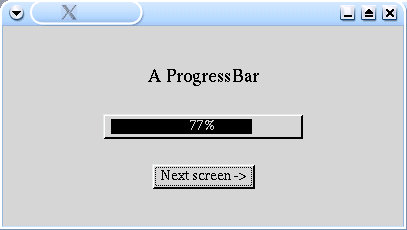
\includegraphics[width=4.2398in,height=2.3953in]{ub-img/ub-img55.jpg}
\end{center}

{\sffamily\bfseries Figure 18-6:}
{\sffamily Progress bar in use}

More complex components use other components within themselves. For
example, the \texttt{TextList} class contains two \texttt{ScrollBar}s,
each of which in turn contains two \texttt{IconButton}s. The
\texttt{Component} class has support for contained objects built in, so
creating components of this sort is quite easy.

Figure 18-7 shows a dialog window containing another example component
which contains an IconButton and a Label as subcomponents. \ A list of
strings is given as an input parameter. When the button is pressed the
label changes to the next item in the list, or goes back to the first
one. \ The user can thus select any of the items.

\begin{center}
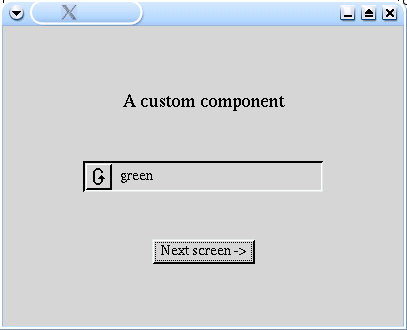
\includegraphics[width=3.4992in,height=2.6543in]{ub-img/ub-img56.jpg}
\end{center}

{\sffamily\bfseries Figure 18-7:}
{\sffamily Circulate component in use}

\bigskip

In this example, sub-components \texttt{b} and \texttt{l} are
initialized in the component's constructor, and
added to the component using the \texttt{add} method. This ensures
they are properly initialized. A listener is connected to the button
so that the selection moves on one when it is pressed. The
\texttt{set\_selection()} method is available to a client program to
change the selection programmatically. Note how this method invokes
\texttt{invalidate()}. This tells the toolkit that the component
needs to be re-displayed. To keep the GUI responsive, the toolkit
will only schedule this re-display when there are no user input events
to be processed. So, \texttt{invalidate()} doesn't
actually invoke the component's \texttt{display()}
method directly.

The \texttt{resize()} method sets the sub-components'
position and size, and then calls the \texttt{resize()} method for each
of them. The \texttt{display()} method erases the
component's rectangular area, draws a border, and
draws the two sub-components into the area. The \texttt{set\_one()}
method is also overridden to provide some custom attributes for the
component. For all other attributes, the parent
class's \texttt{set\_one()} method is invoked, meaning
all the standard attributes work too. So, a client can construct a
\texttt{Circulate} with something like :

\iconcode{
\>   \ c := Circulate("size=,250",
"pos=20,20", \\
\>   \ \ \ \ \ \ \ \ \ \ \ \ \ \ \ \ \ \ \ \ \ \ \ "selection\_list=hot,warm,cold",
"selection=2",
"bg=green")
}

Note how the height is omitted; the \texttt{resize()} method will set a
default value.

\bigskip

{\sffamily\bfseries Listing 18-7}

{\sffamily\bfseries Circulate component}

\iconcode{
package gui \\
link graphics \\
\ \\
\$include "guih.icn" \\
\ \\
\# \\
\# Selection from a list \\
\# \\
class Circulate : Component(selection, selection\_list, b, l) \\
\>   \# \\
\>   \# Set the list from which selections are made. \\
\>   \# \\
\>   \# @param x the list of selection strings \\
\>   method set\_selection\_list(x) \\
\>   \ \ \ selection\_list := x \\
\>   \ \ \ set\_selection(1) \\
\>   \ \ \ return x \\
\>   end \\
\ \\
\>   \# \\
\>   \# Set the selection to the given index into the selection list. \\
\>   \# \\
\>   \# @param x an index into the selection list \\
\>   method set\_selection(x) \\
\>   \ \ \ selection := x \\
\>   \ \ \ l.set\_label(selection\_list[selection]) \\
\>   \ \ \ invalidate() \\
\>   \ \ \ return x \\
\>   end \\
\ \\
\>   \# \\
\>   \# Return the current selection, as an index in the selection list. \\
\>   \# \\
\>   \# @return an integer, being the current selection \\
\>   method get\_selection() \\
\>   \ \ \ return selection \\
\>   end \\
\ \\
\>   \# \\
\>   \# Called once at startup, and whenever the window is resized. \\
\>   \# \\
\>   method resize() \\
\>   \ \ \ /h\_spec := WAttrib(cwin, "fheight") + 16 \\
\>   \ \ \ compute\_absolutes() \\
\ \\
\>   \ \ \ \# \\
\>   \ \ \ \# Set button position and size \\
\>   \ \ \ b.set\_pos(BORDER\_WIDTH, BORDER\_WIDTH) \\
\>   \ \ \ b.set\_size(h - 2 * BORDER\_WIDTH, h - 2 * BORDER\_WIDTH) \\
\>   \ \ \ b.resize() \\
\ \\
\>   \ \ \ l.set\_pos(h - BORDER\_WIDTH +
DEFAULT\_TEXT\_X\_SURROUND, h / 2) \\
\>   \ \ \ l.set\_align("l",
"c") \\
\>   \ \ \ l.set\_size(w - h - 2 *
DEFAULT\_TEXT\_X\_SURROUND, \\
\>   \ \ \ \ \ \ \ \ \ \ \ \ \ \ \ \ \ \ \ h - 2 * BORDER\_WIDTH) \\
\>   \ \ \ l.resize() \\
\>   \ \ \ return \\
\>   end \\
\ \\
\>   \# \\
\>   \# Display the object. \ In this case, double buffering is not necessary.\\
\>   \# \\
\>   method display(buffer\_flag) \\
\>   \ \ \ W := if /buffer\_flag then cwin else cbwin \\
\>   \ \ \ EraseRectangle(W, x, y, w, h) \\
\>   \ \ \ DrawSunkenRectangle(W, x, y, w, h) \\
\>   \ \ \ l.display(buffer\_flag) \\
\>   \ \ \ b.display(buffer\_flag) \\
\>   \ \ \ do\_shading(W) \\
\>   end \\
\ \\
\>   \# \\
\>   \# The handler for the button - move the selection forward. \\
\>   \# \\
\>   method on\_button\_pressed(ev) \\
\>   \ \ \ set\_selection(1 + selection \% *selection\_list) \\
\>   \ \ \ create\_event\_and\_fire(SELECTION\_CHANGED\_EVENT, e) \\
\>   end \\
\ \\
\>   method set\_one(attr, val) \\
\>   \ \ \ case attr of \{ \\
\>   \ \ \ \ \ \ "selection" :
set\_selection(int\_val(attr, val)) \\
\>   \ \ \ \ \ \ "selection\_list" :
set\_selection\_list(val) \\
\>   \ \ \ \ \ \ default: self.Component.set\_one(attr, val) \\
\>   \ \ \ \} \\
\>   end \\
\ \\
\>   initially(a[])  \\
\>   \ \ \ self.Component.initially() \\
\>   \ \ \ l := Label() \\
\>   \ \ \ l.clear\_draw\_border() \\
\>   \ \ \ add(l) \\
\>   \ \ \ b := IconButton() \\
\>   \ \ \ b.connect(self,
"on\_button\_pressed", ACTION\_EVENT) \\
\>   \ \ \ add(b) \\
\>   \ \ \ b.set\_draw\_border() \\
\>   \ \ \ b.set\_img("13,c1,\~{}\~{}\~{}\~{}0000\~{}\~{}\~{}\~{}\~{}\_ \\
\>\>\~{}\~{}\~{}000000\~{}\~{}\~{}\~{}\~{}\~{}00\~{}\~{}\~{}\~{}00\~{}\~{}\~{}\~{}00\~{}\~{}\~{}\~{}\~{}\~{}00\~{}\~{}\_ \\
\>\>\~{}00\~{}\~{}\~{}\~{}\~{}\~{}00\~{}\~{}\~{}00\~{}\~{}\~{}\~{}\~{}\~{}\~{}\~{}\~{}\~{}\~{}00\~{}\~{}\~{}\~{}\~{}\~{}\~{}\~{}\~{}\~{}\_ \\
\>\>\~{}00\~{}\~{}\~{}\~{}\~{}\~{}0\~{}\~{}\~{}\~{}00\~{}\~{}\~{}\~{}\~{}000\~{}\~{}\~{}00\~{}\~{}\~{}\~{}00000\~{}\_ \\
\>\>\~{}00\~{}\~{}\~{}0000000\~{}00\~{}\~{}\~{}\~{}\~{}\~{}00\~{}\~{}\~{}00\~{}\~{}\~{}\~{}\~{}\~{}00\~{}\~{}\_ \\
\>\>\~{}00\~{}\~{}\~{}\~{}\~{}\~{}00\~{}\~{}\~{}\~{}00\~{}\~{}\~{}\~{}00\~{}\~{}\~{}\~{}\~{}\~{}000000\~{}\~{}\~{}\~{}\_ \\
\>\>\~{}\~{}\~{}\~{}0000\~{}\~{}\~{}\~{}\~{}") \\
\>   \ \ \ set\_fields(a) \\
end
}

\subsection*{Customized menu components}

Listing 18-8 contains a custom menu component. The class hierarchy for
menu structures is different to other components, and so this component
is a \index{subclass}subclass of \texttt{SubMenu}, rather than
\texttt{Component}. The component allows the user to select one of a
number of colors from a Palette by clicking on the desired box.
Again, please read this example in conjunction with the reference
section on menus.

\bigskip

{\sffamily\bfseries Listing 18-8}

{\sffamily\bfseries Color Palette Program}

\iconcode{
import gui \\
\ \\
\# \\
\# Include the standard constants. Define width of one colour cell in pixels.\\
\# \\
\$include "guih.icn" \\
\$define CELL\_WIDTH 30 \\
\ \\
class Palette : SubMenu( \\
\>   w, h, \ \ \ \ \ \ \ \ \ \ \ \ \ \ \ \ \ \ \ \# width and height \\
\>   colour, \ \ \ \ \ \ \ \ \ \ \ \ \ \ \ \ \# Color number selected \\
\>   palette, \ \ \ \ \ \ \ \ \ \ \ \ \ \ \ \# List of colors \\
\>   box\_size, \ \ \ \ \ \ \ \ \ \ \ \ \# Width/height in cells \\
\>   temp\_win \ \ \ \ \ \ \ \ \ \ \ \ \# Temporary window \\
\>   ) \\
\ \\
\>   \# \\
\>   \# Get the result \\
\>   \# \\
\>   method get\_colour() \\
\>   \ \ \ return palette[colour] \\
\>   end \\
\ \\
\>   \# \\
\>   \# Set the palette list \\
\>   \# \\
\>   method set\_palette(l) \\
\>   \ \ \ box\_size := integer(sqrt(*l)) \\
\>   \ \ \ return palette := l \\
\>   end \\
\ \\
\>   \# \\
\>   \# This is called by the toolkit; it is a convenient place to initialize sizes. \\
\>   \# \\
\>   method resize() \\
\>   \ \ \ w := h := box\_size * CELL\_WIDTH + 2 * BORDER\_WIDTH \\
\>   end \\
\ \\
\>   \# \\
\>   \# Called to display the item. \ The x, y co-ordinates have been set up \\
\>   \# for us and give the top left hand corner of the display.  \\
\>   \# \\
\>   method display() \\
\>   \ \ \ if /temp\_win then \{ \\
\>   \ \ \ \ \ \ \# \\
\>   \ \ \ \ \ \ \# Open a temporary area for the menu and copy. \\
\>   \ \ \ \ \ \ temp\_win := WOpen("canvas=hidden",
                                    "size=" {\textbar}{\textbar} w
                            {\textbar}{\textbar} "," {\textbar}{\textbar} h) \\
\>   \ \ \ \ \ \ CopyArea(parent\_component.get\_parent\_win(), \\
\>   \ \ \ \ \ \ \ \ \ \ \ \ \ \ \ temp\_win, x, y, w, h, 0, 0) \\
\>\>   \} \\
\ \\
\>   \ \ \ cw := Clone(parent\_component.cwin) \\
\ \\
\>   \ \ \ \# \\
\>   \ \ \ \# Clear area and draw rectangle around whole, then draw the color grid \\
\>   \ \ \ EraseRectangle(cw, x, y, w, h) \\
\>   \ \ \ DrawRaisedRectangle(cw, x, y, w, h) \\
\>   \ \ \ y1 := y + BORDER\_WIDTH \ \ \ \ \  \\
\>   \ \ \ e := create "fg=" {\textbar}{\textbar} !palette \\
\>   \ \ \ every 1 to box\_size do \{ \\
\>   \ \ \ \ \ \ x1 := x + BORDER\_WIDTH \  \\
\>   \ \ \ \ \ \ every 1 to box\_size do \{ \\
\>   \ \ \ \ \ \ \ \ \ WAttrib(cw, @e) \\
\>   \ \ \ \ \ \ \ \ \ FillRectangle(cw, x1, y1, CELL\_WIDTH, CELL\_WIDTH) \\
\>   \ \ \ \ \ \ \ \ \ x1 +:= CELL\_WIDTH \\
\>   \ \ \ \ \ \ \} \\
\>   \ \ \ \ \ \ y1 +:= CELL\_WIDTH \\
\>   \ \ \ \} \\
\>   \ \ \ Uncouple(cw) \\
\>   end \\
\ \\
\>   \# \\
\>   \# Test whether pointer in palette\_region, and if so which cell it's in \\
\>   \# \\
\>   method in\_palette\_region() \\
\>   \ \ \ if (x {\textless}= \&x {\textless} x + w) \& (y {\textless}= \&y {\textless} y + h)
then \{ \\
\>   \ \ \ \ \ \ x1 := (\&x - x - BORDER\_WIDTH) / CELL\_WIDTH \\
\>   \ \ \ \ \ \ y1 := (\&y - y - BORDER\_WIDTH) / CELL\_WIDTH \\
\>   \ \ \ \ \ \ return 1 + x1 + y1 * box\_size \\
\>\>   \} \\
\>   end \\
\ \\
\>   \# \\
\>   \# Will be called if our menu is open. \\
\>   \# \\
\>   method handle\_event(e) \\
\>   \ \ \ if i := in\_palette\_region() then \{ \\
\>   \ \ \ \ \ \ if integer(e) = (\&lrelease {\textbar} \&rrelease {\textbar}
                                  \&mrelease) then \{ \\
\>   \ \ \ \ \ \ \ \ \ colour := i \\
\>   \ \ \ \ \ \ \ \ \ \# This is a helper method in the superclass which \\
\>   \ \ \ \ \ \ \ \ \ \# closes the menu system and fires an ACTION\_EVENT \\
\>   \ \ \ \ \ \ \ \ \ succeed(e) \\
\>   \ \ \ \ \ \ \} \\
\>   \ \ \ \} else \{ \\
\>   \ \ \ \ \ \ if integer(e) = (\&lrelease {\textbar} \&rrelease
{\textbar} \&mrelease {\textbar} \\
\>   \ \ \ \ \ \ \ \ \ \ \ \ \ \ \ \ \ \ \ \ \ \ \ \&lpress {\textbar}
\&rpress {\textbar} \&mpress) then \\
\>   \ \ \ \ \ \ \ \ \ \# This is a helper method in the superclass
which \\
\>   \ \ \ \ \ \ \ \ \ \# closes the menu system, without firing an
event. \\
\>   \ \ \ \ \ \ \ \ \ close\_all() \\
\>   \ \ \ \} \\
\>   end \\
\ \\
\>   \# \\
\>   \# Close this menu. Restore window area. \\
\>   \# \\
\>   method hide() \\
\>   \ \ \ EraseRectangle(parent\_component.cwin, x, y, w, h) \\
\>   \ \ \ CopyArea(temp\_win, parent\_component.get\_parent\_win(),
                    0, 0, w, h, x, y) \\
\>   \ \ \ WClose(temp\_win) \\
\>   \ \ \ temp\_win := \&null \\
\>   end \\
\ \\
\>   \# Support a "palette" attrib \\
\>   method set\_one(attr, val) \\
\>   \ \ \ case attr of \{ \\
\>   \ \ \ \ \ \ "palette" :
set\_palette(val) \\
\>   \ \ \ \ \ \ default : self.MenuComponent.set\_one(attr, val) \\
\>   \ \ \ \ \ \ \} \\
\>   end \\
\ \\
\>   initially(a[]) \\
\>   \ \ \ self.SubMenu.initially() \\
\>   \ \ \ \# \\
\>   \ \ \ \# Set the image to appear on the Menu above ours. We could design a tiny \\
\>   \ \ \ \# icon and use that instead of the standard arrow if we wished. \\
\>   \ \ \ \# Call set\_fields to support the attrib style constructor. \\
\>   \ \ \ \#  \\
\>   \ \ \ set\_img\_right(img\_style("arrow\_right")) \\
\>   \ \ \ set\_fields(a) \\
end \\
\ \\
\# \\
\# Test class dialog. \\
\# \\
class TestPalette : Dialog(palette) \\
\>   method on\_palette(ev) \\
\>   \ \ \ write("Colour selected : "
{\textbar}{\textbar} palette.get\_colour()) \\
\>   end \\
\ \\
\>   method on\_anything(ev) \\
\>   \ \ \ write("Anything item selected") \\
\>   end \\
\ \\
\>   method component\_setup() \\
\>   \ \ \ local menu\_bar, menu, text\_menu\_item, close \\
\>   \ \ \ attrib("size=400,200") \\
\ \\
\>   \ \ \ \# \\
\>   \ \ \ \# Create a MenuBar which includes our palette as a sub-menu \\
\>   \ \ \ menu\_bar := MenuBar("pos=0,0") \\
\>   \ \ \ menu := Menu("label=Test") \\
\>   \ \ \ text\_menu\_item := TextMenuItem("label=Anything") \\
\>   \ \ \ text\_menu\_item.connect(self, "on\_anything", ACTION\_EVENT) \\
\>   \ \ \ menu.add(text\_menu\_item) \\
\ \\
\>   \ \ \ palette := Palette("label=Test menu", \\
\>   \ \ \ \ \ \ \ \ \ \ \ \ \ \ \ \ \ \ \ \ \ \ "palette=red,green,yellow,black,white,purple,gray,blue,pink") \\
\>   \ \ \ palette.connect(self, "on\_palette", ACTION\_EVENT) \\
\>   \ \ \ menu.add(palette) \\
\>   \ \ \ menu\_bar.add(menu) \\
\>   \ \ \ add(menu\_bar) \\
\ \\
\>   \ \ \ \# \\
\>   \ \ \ \# Add a close button.\\
\>   \ \ \ close := TextButton("pos=50\%,66\%", "align=c,c", "label=Close") \\
\>   \ \ \ close.connect(self, "dispose", ACTION\_EVENT) \\
\>   \ \ \ add(close) \\
\>   end \\
end \\
\ \\
procedure main() \\
\>   TestPalette().show\_modal() \\
end
}

\bigskip

The resulting window, with the \texttt{Palette} menu active is shown in
Figure 18-8.

\begin{center}
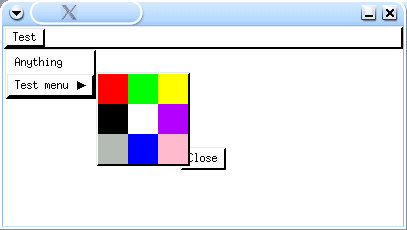
\includegraphics[width=4.2398in,height=2.3953in]{ub-img/ub-img57.jpg}
\end{center}

{\sffamily\bfseries Figure 18-8:}
{\sffamily TestPalette window}

\subsection*{Tickers}

GUI programs spend most of their time waiting for user input
events. The toolkit allows this spare time to be exploited by user
programs by the use of "tickers". \ These
are classes which subclass \texttt{Ticker}, and\texttt{ }implement a
single method, \texttt{tick()}, which is invoked at a specified
interval. If the toolkit is busy processing events or
updating the display, the actual interval may be much greater than that
requested, but it will never be less.

Many components make use of tickers. For example when the mouse button
is dragged below the bottom of an \texttt{EditableTextList} and held,
the cursor scrolls downwards without any user events occurring. This
is handled with a simple ticker:

\iconcode{
class FirstTicker : Ticker() \\
\>   method tick() \\
\>   \ \ \ write("Doing something in
FirstTicker") \\
\>   end \\
end
}

\noindent
If we had an instance \texttt{t} of this ticker, we would start it with:

\iconcode{
t.set\_ticker(1000)}

\noindent and stop it with

\iconcode{
t.stop\_ticker()}

Both calls would have to be made whilst a dialog was open, because it is
from within the toolkit's event processing loop that
tickers are scheduled.

For convenience, the base \texttt{Component} class is a subclass of
\texttt{Ticker}. This means that a dialog class (which is itself a
subclass of \texttt{Component}, and hence of \texttt{Ticker} too), can
simply implement a \texttt{tick()} method to use the ticker facility.
It simply needs to invoke \texttt{set\_ticker()} and
\texttt{stop\_ticker()} to start and stop the ticker, respectively.
Another method, \texttt{retime\_ticker()}, allows the rate of an
active ticker to be changed.

One important rule regarding ticker programming has to be borne in mind,
and that is that the \texttt{tick()} method implementation must return
quite quickly; at most within a few tenths of a second. If it does
not, then the GUI may become unresponsive to user events, which cannot
be processed whilst control is in the \texttt{tick()} method.

The \texttt{tick()} method must return quickly. If the
task you want to implement in the background is by nature deeply
structured and takes a long time, it may be difficult
to get out of the \texttt{tick()} method promptly and continue in the
same state on the next tick.  Co-expressions can
be helpful here. A co-expression
maintains its own stack and can suspend itself, and then
continue again later with the state (including stack) intact.

Here is an example program which illustrates these points. It
generates prime numbers using the Erastothenes' sieve
method, in a ticker, using a co-expression to conveniently suspend
generation after each prime.
This program also introduces a new component, a slider which is
used to increase or decrease the ticker rate dynamically.

{\sffamily\bfseries
Listing 18-9}

{\sffamily\bfseries
Erastothenes' Sieve Program}

\iconcode{
import gui \\
\$include "guih.icn" \\
\$define PRIME\_LIMIT 20000 \\
\ \\
\# \\
\# A program to calculate prime numbers in a background ticker, \\
\# and display them in a dialog. \\
\# \\
class Sieve : Dialog(prime\_ce, interval, count\_label, prime\_label,  \\
\>   \ \ \ \ \ \ \ \ \ \ \ \ \ \ \ \ \ \ rate\_label, start, stop) \\
\ \\
\>   \# \\
\>   \# Bring the label and ticker into line with the interval slider. \\
\>   \# If the ticker is running, retime it. \\
\>   \# \\
\>   method synch\_interval() \\
\>   \ \ \ rate\_label.set\_label(interval.get\_value()
{\textbar}{\textbar} " ms") \\
\>   \ \ \ if is\_ticking() then retime\_ticker(interval.get\_value()) \\
\>   end \\
\ \\
\>   \# \\
\>   \# Toggle the grey state of the start/stop buttons. \\
\>   \# \\
\>   method toggle\_buttons() \\
\>   \ \ \ start.toggle\_is\_shaded() \\
\>   \ \ \ stop.toggle\_is\_shaded() \\
\>   end \\
\ \\
\>   \# \\
\>   \# When the start button is pressed, toggle the grey state and start the ticker. \\
\>   \# \\
\>   method on\_start() \\
\>   \ \ \ toggle\_buttons() \\
\>   \ \ \ set\_ticker(interval.get\_value()) \\
\>   end \\
\ \\
\>   \# \\
\>   \# When the stop button is pressed, toggle the grey state and stop the ticker. \\
\>   \#  \\
\>   method on\_stop() \\
\>   \ \ \ toggle\_buttons() \\
\>   \ \ \ stop\_ticker() \\
\>   end \\
\ \\
\>   \# \\
\>   \# The tick method, which is invoked regularly by the toolkit. \\
\>   \# It just invokes the co-expression to display the next prime. \\
\>   \# \\
\>   method tick() \\
\>   \ \ \ @prime\_ce \\
\>   end \\
\ \\
\>   \# \\
\>   \# This method consitutes the co-expression body. \\
\>   \# \\
\>   method primes() \\
\>   \ \ \ local prime\_candidate, non\_prime\_set := set(), prime\_count := 0 \\
\ \\
\>   \ \ \ every prime\_candidate := 2 to \ PRIME\_LIMIT do \{ \\
\>   \ \ \ \ \ \ if not member(non\_prime\_set, prime\_candidate) then
\{ \\
\>   \ \ \ \ \ \ \ \ \ \# \\
\>   \ \ \ \ \ \ \ \ \ \# Update the UI. \\
\>   \ \ \ \ \ \ \ \ \ count\_label.set\_label(prime\_count +:= 1) \\
\>   \ \ \ \ \ \ \ \ \ prime\_label.set\_label(prime\_candidate) \\
\>   \ \ \ \ \ \ \ \ \ \# \\
\>   \ \ \ \ \ \ \ \ \ \# Update the non-prime set. \\
\>   \ \ \ \ \ \ \ \ \ every insert(non\_prime\_set,\\
\>   \ \ \ \ \ \ \ \ \ \ \ \ 2 * prime\_candidate to PRIME\_LIMIT by prime\_candidate) \\
\>   \ \ \ \ \ \ \ \ \ \# \\
\>   \ \ \ \ \ \ \ \ \ \# Suspend the co-expression until the next tick. \\
\>   \ \ \ \ \ \ \ \ \ @\&source \\
\>   \ \ \ \ \ \ \} \\
\>   \ \ \ \} \\
\>   end \\
\ \\
\>   method component\_setup() \\
\>   \ \ \ local prime\_border, rate, buttons, b \\
\ \\
\>   \ \ \ attrib("size=325,200",
"label=Sieve") \\
\>   \ \ \ connect(self, "dispose",
CLOSE\_BUTTON\_EVENT) \\
\ \\
\>   \ \ \ prime\_border :=
Border("pos=20,20",
"size=100\%-40,78") \\
\>   \ \ \ prime\_border.set\_title(Label("pos=10,0",
"label=Primes")) \\
\>   \ \ \ prime\_ce := create primes() \\
\ \\
\>   \ \ \ prime\_border.add(Label("pos=20,18",
"label=Prime:")) \\
\>   \ \ \ count\_label :=
Label("pos=77,18",
"size=40") \\
\>   \ \ \ count\_label.set\_label("") \\
\>   \ \ \ prime\_border.add(count\_label) \\
\>   \ \ \ prime\_border.add(Label("pos=20,40",
"label=Value:")) \\
\>   \ \ \ prime\_label :=
Label("pos=77,40",
"size=40") \\
\>   \ \ \ prime\_label.set\_label("") \\
\>   \ \ \ prime\_border.add(prime\_label) \\
\ \\
\>   \ \ \ add(prime\_border) \\
\ \\
\>   \ \ \ rate := Panel("pos=20,112",
"size=100\%-40,30") \\
\>   \ \ \ rate.add(Label("pos=0,50\%",
"size=45",
"align=l,c",
"label=Rate:")) \\
\>   \ \ \ interval := Slider("pos=45,50\%", "size=100\%-90", "align=l,c", \\

\>   \ \ \ \ \ \ \ \ \ \ \ \ \ \ \ \ \ \ \ \ \ \ "range=20,2020", "is\_horizontal=t") \\
\>   \ \ \ interval.set\_value(1000) \\
\>   \ \ \ interval.connect(self,
"synch\_interval", SLIDER\_DRAGGED\_EVENT) \\
\>   \ \ \ rate.add(interval) \\
\ \\
\>   \ \ \ rate\_label := Label("pos=100\%,50\%", "size=45", "align=r,c", \\
\>\>\>\>"internal\_alignment=r") \\
\>   \ \ \ rate.add(rate\_label) \\
\>   \ \ \ synch\_interval() \\
\>   \ \ \ add(rate) \\
\ \\
\>   \ \ \ buttons := Panel("pos=50\%,158",
"size=161,25",
"align=c,t") \\
\>   \ \ \ start := TextButton("pos=0,0",
"label=Start") \\
\>   \ \ \ start.connect(self, "on\_start",
ACTION\_EVENT) \\
\>   \ \ \ buttons.add(start) \\
\>   \ \ \ stop := TextButton("pos=58,0",
"label=Stop",
"is\_shaded=t") \\
\>   \ \ \ stop.connect(self, "on\_stop",
ACTION\_EVENT) \\
\>   \ \ \ buttons.add(stop) \\
\>   \ \ \ b := TextButton("pos=108,0",
"label=Quit") \\
\>   \ \ \ b.connect(self, "dispose",
ACTION\_EVENT) \\
\>   \ \ \ buttons.add(b) \\
\>   \ \ \ add(buttons) \\
\>   end \\
end \\
\ \\
procedure main() \\
\>   Sieve().show\_modal() \\
end
}

\bigskip

\begin{center}
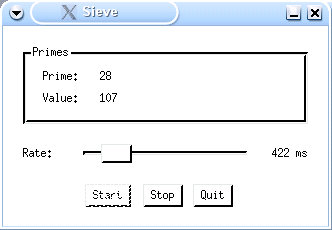
\includegraphics[width=3.4575in,height=2.3953in]{ub-img/ub-img58.jpg}
\end{center}

{\sffamily\bfseries Figure 18-9:}
{\sffamily Sieve}

\section{Advanced List Handling}

Several of the more sophisticated components extend a common base class,
\texttt{SelectableScrollArea}, namely \texttt{TextList}, \texttt{Table}
and \texttt{Tree}. \ (In fact, \texttt{Table} doesn't
directly extend \texttt{SelectableScrollArea,} it contains a header
component and a content component that does). It is quite easy to add
some advanced features to these components, such as right-click popup
menus, multi-selection and drag and drop, and this is explained in this
section.

\subsection*{Selection}

Selection handling is straightforward. First, configure the component
so that it allows selection of no, one, or many rows using the methods
\texttt{set\_select\_none()}, \texttt{set\_select\_one()} or
\texttt{set\_select\_many()}, or the attributes
\texttt{"select\_none"}, \texttt{"select\_one"} or \texttt{"select\_many"}.
Then, listen for changes by listening for a
\texttt{SELECTION\_CHANGED\_EVENT} to be fired :

\iconcode{
\>   comp.connect(self, "handle\_selection", SELECTION\_CHANGED\_EVENT)}

When such an event does occur, the current selections can be retrieved
in one of two ways. \ Either by getting the indexes of the selections
using \texttt{get\_selections()}, or by getting the objects selected,
using \texttt{object\_get\_selections()}. The former returns a list
of integers, the latter a list of objects whose type depends on the
component. \ For a \texttt{TextList}, a list of strings is returned,
for a \texttt{Table}, a list of lists (each being a
row's data), and for a \texttt{Tree}, a list of
\texttt{Node} objects is returned.
There are corresponding setter methods for setting the selection dynamically.


\subsection*{Popups}

Adding popup menus is also easy. First create a \texttt{Popup}
component, ready to be shown. Then, listen for a
\texttt{MOUSE\_RELEASE\_EVENT}. Finally, when an event occurs check
that is a right mouse release, and that the object is in the state you
want. If it is, just activate the popup via its \texttt{popup()}
method.

\subsection*{Drag and drop}

The toolkit supports a limited form of drag and drop, which works only between
components within the same window.
To implement drag and drop, a class, \texttt{DndHandler}, must be
subclassed and an instance "plugged-in" to
the component which is a source or target of a potential drag and drop
operation, using its \texttt{set\_dnd\_handler()} method.
The \texttt{DndHandler} class provides five callback methods which the
toolkit uses to control a drag and drop operation.
When using the \texttt{SelectableScrollArea} family of components, it is
best to subclass \texttt{SelectableScrollAreaDndHandler}, which is a
custom subclass of \texttt{DndHandler}, with several methods already
defined appropriately.

All of the above features are brought together in the following example
program which provides a \texttt{Tree} and a \texttt{TextList}. Drag
and drop is enabled between the two components, and both provide popup
menus for adding/deleting elements.

\bigskip

\bigskip

\begin{center}
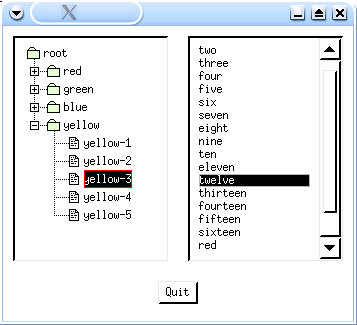
\includegraphics[width=3.7189in,height=3.3846in]{ub-img/ub-img59.jpg}
\end{center}

{\sffamily\bfseries Figure 18-10:}
{\sffamily Drag and drop}

\bigskip

{\sffamily\bfseries Listing 18-10}
{\sffamily\bfseries The Drag and drop Program}

\iconcode{
import gui \\
\$include "guih.icn" \\
\ \\
\# \\
\# A DndHandler for the list \\
\# \\
class ListDndHandler : SelectableScrollAreaDndHandler() \\
\>   \# \\
\>   \# A drop has occurred; we succeed iff we accept it \\
\>   \# \\
\>   method can\_drop(d) \\
\>   \ \ \ local l, ll \\
\>   \ \ \ if l := parent.get\_highlight() then \{ \\
\>   \ \ \ \ \ \ if d.get\_source() === parent then \# Move within the list itself \\
\>   \ \ \ \ \ \ \ \ \ parent.move\_rows(parent.get\_gesture\_selections(), l) \\
\>   \ \ \ \ \ \ else \{ \\
\>   \ \ \ \ \ \ \ \ \ \# \\
\>   \ \ \ \ \ \ \ \ \ \# Copy from tree to list. d.get\_content() gives \\
\>   \ \ \ \ \ \ \ \ \ \# a list of the nodes being dragged. \\
\>   \ \ \ \ \ \ \ \ \ ll := [ ] \\
\>   \ \ \ \ \ \ \ \ \ every el := !d.get\_content() do \# Don't drag folders. \\
\>   \ \ \ \ \ \ \ \ \ \ \ \ if /el.is\_folder\_flag then put(ll, el.get\_label()) \\
\>   \ \ \ \ \ \ \ \ \ parent.insert\_rows(ll, l) \\
\>   \ \ \ \ \ \ \} \\
\>   \ \ \ \ \ \ return \\
\>   \ \ \ \} \\
\>   end \\
\ \\
\>   \# \\
\>   \# This is invoked after a successful operation when the \\
\>   \# list was the source. \ If the destination (c)
wasn't the \\
\>   \# list, then we must delete the rows from the list. \\
\>   \# \\
\>   method end\_drag(d, c) \\
\>   \ \ \ if c \~{}=== parent then \\
\>   \ \ \ \ \ \ parent.delete\_rows(parent.get\_gesture\_selections()) \\
\>   end \\
end \\
\ \\
\# \\
\# A DndHandler for the tree \\
\# \\
class TreeDndHandler : SelectableScrollAreaDndHandler() \\
\>   \# \\
\>   \# Called during a drag event. We succeed iff the user is dragging over \\
\>   \# a row (this is handled by the parent) AND the thing we're over is a folder. \\
\>   \# \\
\>   method drag\_event(d) \\
\>   \ \ \ if SelectableScrollAreaDndHandler.drag\_event(d) then \\
\>   \ \ \ \ \ \ return
{\textbackslash}(parent.object\_get\_highlight().is\_folder\_flag) \\
\>   end \\
\ \\
\>   \# \\
\>   \# A drop has occurred; we succeed iff we accept it. \\
\>   \# Only consider a drop on a folder. \\
\>   \# \\
\>   method can\_drop(d) \\
\>   \ \ \ local s, other, n, el \\
\>   \ \ \ if other := parent.object\_get\_highlight() \&
{\textbackslash}other.is\_folder\_flag then \{ \\
\>   \ \ \ \ \ \ if d.get\_source() === parent then \{ \\
\>   \ \ \ \ \ \ \ \ \ \# \\
\>   \ \ \ \ \ \ \ \ \ \# If parent is the drop source, then we have a dnd
                          from within \\
\>   \ \ \ \ \ \ \ \ \ \# the tree. So, we just move the nodes. \\
\>   \ \ \ \ \ \ \ \ \ \# d.get\_content() will be a list of the nodes
that were dragged. \\
\>   \ \ \ \ \ \ \ \ \ every el := !d.get\_content() do \{ \\
\>   \ \ \ \ \ \ \ \ \ \ \ \ if el.get\_parent\_node().delete\_node(el)
then \\
\>   \ \ \ \ \ \ \ \ \ \ \ \ \ \ \ other.add(el) \\
\>   \ \ \ \ \ \ \ \ \ \} \\
\>   \ \ \ \ \ \ \} else \{ \\
\>   \ \ \ \ \ \ \ \ \ \# \\
\>   \ \ \ \ \ \ \ \ \ \# Drop from list. \ In this case d.get\_content() will be a list of strings. \\
\>   \ \ \ \ \ \ \ \ \ every el := !d.get\_content() do \{ \\
\>   \ \ \ \ \ \ \ \ \ \ \ \ n := TreeNode() \\
\>   \ \ \ \ \ \ \ \ \ \ \ \ n.set\_label(el) \\
\>   \ \ \ \ \ \ \ \ \ \ \ \ other.add(n) \\
\>   \ \ \ \ \ \ \ \ \ \} \\
\>   \ \ \ \ \ \ \} \\
\>   \ \ \ \ \ \ \# \\
\>   \ \ \ \ \ \ \# Notify the tree that the node data structure has altered. \\
\>   \ \ \ \ \ \ parent.tree\_structure\_changed() \\
\>   \ \ \ \ \ \ return \\
\>   \ \ \ \} \\
\>   end \\
\ \\
\>   \# \\
\>   \# This is invoked after a successful operation when the tree was the source.\\
\>   \# If the destination (c) wasn't the tree, we must delete the nodes from the tree. \\
\>   \# \\
\>   method end\_drag(d, c) \\
\>   \ \ \ if c \~{}=== parent then \{ \\
\>   \ \ \ \ \ \ \# \\
\>   \ \ \ \ \ \ \# Delete all the nodes which will have been dragged. \\
\>   \ \ \ \ \ \ every n := !parent.object\_get\_gesture\_selections() do \\
\>   \ \ \ \ \ \ \ \ \ if /n.is\_folder\_flag then \\
\>   \ \ \ \ \ \ \ \ \ \ \ \ n.get\_parent\_node().delete\_node(n) \\
\>   \ \ \ \ \ \ \# \\
\>   \ \ \ \ \ \ \# Notify the tree that the node data structure has altered. \\
\>   \ \ \ \ \ \ parent.tree\_structure\_changed() \\
\>   \ \ \ \} \\
\>   end \\
end \\
\ \\
\# \\
\# We use a custom Node subclass to also store an
"is\_folder\_flag" flag. \\
\# \\
class TreeNode : Node(is\_folder\_flag) \\
initially \\
\>   self.Node.initially() \\
\>   if {\textbackslash}is\_folder\_flag then \\
\>   \ \ \ set\_bmps([img\_style("closed\_folder"), \\
\>   \ \ \ \ \ \ \ \ \ \ \ \ img\_style("closed\_folder"),
img\_style("closed\_folder")]) \\
end \\
\ \\
\# \\
\# The main dialog. \\
\# \\
class DNDTest : Dialog(tree, lst, tree\_popup, list\_popup, new\_folder\_menu\_item,  \\
\>   \ \ \ \ \ \ \ \ \ \ \ \ \ \ \ \ \ \ \ \ delete\_node\_menu\_item, delete\_rows\_menu\_item) \\
\ \\
\>   \# \\
\>   \# Delete nodes handler \\
\>   \# \\
\>   method on\_delete\_node() \\
\>   \ \ \ local n, i, l \\
\ \\
\>   \ \ \ every n := !(tree.object\_get\_gesture\_selections()) do \\
\>   \ \ \ \ \ \ n.get\_parent\_node().delete\_node(n) \\
\ \\
\>   \ \ \ tree.tree\_structure\_changed() \# Notify tree of the change.\\
\>   end \\
\ \\
\>   \# \\
\>   \# Create a new folder \\
\>   \# \\
\>   method on\_new\_folder() \\
\>   \ \ \ local n, o \\
\ \\
\>   \ \ \ \# \\
\>   \ \ \ \# Simply add a new node under the cursor, and notify the \\
\>   \ \ \ \# tree that the data structure changed. \\
\>   \ \ \ \# \\
\>   \ \ \ if o := tree.object\_get\_cursor() then \{ \\
\>   \ \ \ \ \ \ n := TreeNode(1) \\
\>   \ \ \ \ \ \ n.set\_label("New
folder") \\
\>   \ \ \ \ \ \ o.add(n) \\
\>   \ \ \ \ \ \ tree.tree\_structure\_changed() \\
\>   \ \ \ \ \ \ \} \\
\>   end \\
\ \\
\>   \# \\
\>   \# Delete rows from the list \\
\>   \# \\
\>   method on\_delete\_rows() \\
\>   \ \ \ lst.delete\_rows(lst.get\_gesture\_selections()) \\
\>   end \\
\ \\
\>   \# \\
\>   \# Add some rows to the list, at the cursor position, or at \\
\>   \# the top if there is no cursor. \\
\>   \# \\
\>   method on\_new\_rows() \\
\>   \ \ \ lst.insert\_rows(["new1",
"new2",
"new3"], lst.get\_cursor() {\textbar} 1) \\
\>   end \\
\ \\
\>   \# \\
\>   \# Helper method to create a tree structure. \\
\>   \# \\
\>   method create\_tree() \\
\>   \ \ \ local r := TreeNode(1), n \\
\>   \ \ \ r.set\_label("root") \\
\ \\
\>   \ \ \ every s := ("red" {\textbar}
"green" {\textbar}
"blue" {\textbar}
"yellow") do \{ \\
\>   \ \ \ \ \ \ n := TreeNode(1) \\
\>   \ \ \ \ \ \ n.set\_label(s) \\
\>   \ \ \ \ \ \ r.add(n) \\
\>   \ \ \ \ \ \ every t := 1 to 5 do \{ \\
\>   \ \ \ \ \ \ \ \ \ o := TreeNode() \\
\>   \ \ \ \ \ \ \ \ \ o.set\_label(s {\textbar}{\textbar}
"-" {\textbar}{\textbar}t) \\
\>   \ \ \ \ \ \ \ \ \ n.add(o) \\
\>   \ \ \ \ \ \ \ \ \ \} \\
\>   \ \ \ \ \ \ \} \\
\>   \ \ \ return r \\
\>   end \\
\ \\
\>   \# \\
\>   \# A selection-up event on the tree \\
\>   \# \\
\>   method on\_tree\_release(ev) \\
\>   \ \ \ local n \\
\>   \ \ \ \# \\
\>   \ \ \ \# If the Icon event was a right mouse release, display the popup at the cursor. \\
\>   \ \ \ if ev.get\_param() === \&rrelease then \{ \\
\>   \ \ \ \ \ \ n := tree.object\_get\_cursor() {\textbar} fail \\
\>   \ \ \ \ \ \ \# \\
\>   \ \ \ \ \ \ \# Adjust the shading depending on the node type. \\
\>   \ \ \ \ \ \ if /n.is\_folder\_flag then \\
\>   \ \ \ \ \ \ \ \ \ new\_folder\_menu\_item.set\_is\_shaded() \\
\>   \ \ \ \ \ \ else \\
\>   \ \ \ \ \ \ \ \ \ new\_folder\_menu\_item.clear\_is\_shaded() \\
\>   \ \ \ \ \ \ if n === tree.get\_root\_node() then \\
\>   \ \ \ \ \ \ \ \ \ delete\_node\_menu\_item.set\_is\_shaded() \\
\>   \ \ \ \ \ \ else \\
\>   \ \ \ \ \ \ \ \ \ delete\_node\_menu\_item.clear\_is\_shaded() \\
\>   \ \ \ \ \ \ tree\_popup.popup() \\
\>   \ \ \ \} \\
\>   end \\
\ \\
\>   \# \\
\>   \# A mouse release event on the list \\
\>   \# \\
\>   method on\_list\_release(ev) \\
\>   \ \ \ if ev.get\_param() === \&rrelease then \{ \\
\>   \ \ \ \ \ \ \# \\
\>   \ \ \ \ \ \ \# If some rows to delete... \\
\>   \ \ \ \ \ \ if lst.get\_gesture\_selections() then \\
\>   \ \ \ \ \ \ \ \ \ delete\_rows\_menu\_item.clear\_is\_shaded() \\
\>   \ \ \ \ \ \ else \\
\>   \ \ \ \ \ \ \ \ \ delete\_rows\_menu\_item.set\_is\_shaded() \\
\ \\
\>   \ \ \ \ \ \ list\_popup.popup() \\
\>   \ \ \ \} \\
\>   end \\
\ \\
\>   method component\_setup() \\
\>   \ \ \ local m, quit, mi \\
\>   \ \ \ attrib("size=350,295", "resize=on") \\
\>   \ \ \ connect(self, "dispose", CLOSE\_BUTTON\_EVENT) \\
\>   \ \ \ tree := Tree("pos=50\%-10,10", "size=50\%-20,100\%-70", \\
\>   \ \ \ \ \ \ \ \ \ \ \ \ \ \ \ \ "align=r,t", "select\_many",
"show\_root\_handles=f") \\
\>   \ \ \ tree.set\_root\_node(create\_tree()) \\
\>   \ \ \ tree.set\_dnd\_handler(TreeDndHandler(tree)) \\
\>   \ \ \ tree.connect(self, "on\_tree\_release", MOUSE\_RELEASE\_EVENT) \\
\>   \ \ \ add(tree) \\
\>   \ \ \ quit := TextButton("pos=50\%,100\%-40", "align=c,t", "label=Quit") \\
\>   \ \ \ quit.connect(self, "dispose", ACTION\_EVENT) \\
\>   \ \ \ add(quit) \\
\>   \ \ \ \# Create a TextList, with some arbitrary content. \\
\>   \ \ \ lst := TextList("pos=50\%+10,10", "size=50\%-20,100\%-70",
"select\_many", \\
\>   \ \ \ \ \ \ \ \ \ \ \ \ \ \ \ \ \ \ \ "contents=one,two,three,four,five,six,seven,eight,nine,ten,eleven,\_ \\
\>   \ \ \ \ \ \ \ \ \ \ \ \ \ \ \ \ \ \ \ \ twelve,thirteen,fourteen,fifteen,sixteen,red,blue,green") \\
\>   \ \ \ lst.connect(self, "on\_list\_release", MOUSE\_RELEASE\_EVENT) \\
\>   \ \ \ lst.set\_dnd\_handler(ListDndHandler(lst)) \\
\>   \ \ \ add(lst) \\
\>   \ \ \ tree\_popup := PopupMenu() \\
\>   \ \ \ m := Menu() \\
\>   \ \ \ tree\_popup.set\_menu(m) \\
\>   \ \ \ delete\_node\_menu\_item := TextMenuItem("label=Delete") \\
\>   \ \ \ delete\_node\_menu\_item.connect(self, "on\_delete\_node",
                                            ACTION\_EVENT) \\
\>   \ \ \ m.add(delete\_node\_menu\_item) \\
\>   \ \ \ new\_folder\_menu\_item := TextMenuItem("label=New folder") \\
\>   \ \ \ new\_folder\_menu\_item.connect(self, "on\_new\_folder",
                                           ACTION\_EVENT) \\
\>   \ \ \ m.add(new\_folder\_menu\_item) \\
\>   \ \ \ add(tree\_popup) \\
\>   \ \ \ list\_popup := PopupMenu() \\
\>   \ \ \ m := Menu() \\
\>   \ \ \ list\_popup.set\_menu(m) \\
\>   \ \ \ delete\_rows\_menu\_item := TextMenuItem("label=Delete") \\
\>   \ \ \ delete\_rows\_menu\_item.connect(self, "on\_delete\_rows",
                                            ACTION\_EVENT) \\
\>   \ \ \ m.add(delete\_rows\_menu\_item) \\
\>   \ \ \ mi := TextMenuItem("label=Insert rows") \\
\>   \ \ \ mi.connect(self, "on\_new\_rows", ACTION\_EVENT) \\
\>   \ \ \ m.add(mi) \\
\>   \ \ \ add(list\_popup) \\
\>   end \\
end \\
\ \\
procedure main() \\
\>   DNDTest().show\_modal() \\
end
}

\section{Programming Techniques}

Some of the earlier example dialogs were effectively
``application windows.'' In other words, the
top-level window of a program. This section looks at some techniques
for integrating dialog windows that are secondary or helper windows
into a program.

\subsection*{Parameters}

A dialog window will normally have parameters that the calling program will want
to pass to it before it is displayed using the \texttt{show()} method. Possibly
the attribute syntax \texttt{"key=val"} should be
supported, and perhaps a default value should be set. \ All of these things are
easily supported by following the following structure:

\iconcode{
class AnyDialog : Dialog(a\_variable) \\
\>   method set\_a\_variable(x) \\
\>   \ \ \ a\_variable := x \\
\>   end \\
\>   ... \\
\>   method set\_one(attr, val) \\
\>   \ \ \ case attr of \{ \\
\>   \ \ \ \ \ \ "a\_variable" : \\
\>   \ \ \ \ \ \ \ \ \ set\_a\_variable(string\_val(attr, val)) \\
\>   \ \ \ \ \ \ default: self.Dialog.set\_one(attr, val) \\
\>   \ \ \ \} \\
\>   end \\
\ \\
\>   method component\_setup() \\
\>   \ \ \ \# Initialize Components, possibly depending upon the value of a\_variable \\
\>   \ \ \ ... \\
\>   \ \ \ \# Configure the window itself... \\
\>   \ \ \ attrib("size=300,200") \\
\>   end \\
\ \\
\>   initially(a[]) \\
\>   \ \ \ self.Dialog.initially() \\
\>   \ \ \ a\_variable := "default value" \\
\>   \ \ \ set\_fields(a) \\
end
}

You then use the following code in the calling program:

\iconcode{
\>   d := AnyDialog() \\
\>   d.set\_a\_variable("something")
}

or

\iconcode{
\>   d :=
AnyDialog("a\_variable=something")}

or just

\iconcode{
\>   d := AnyDialog()}

\noindent to use the default for \texttt{a\_variable}. \ Furthermore, the standard
dialog attributes can still be used as you would expect :

\iconcode{
\>   d :=
AnyDialog("a\_variable=something",
"font=times",
"bg=green",
"fg=red")}

Subclassing can follow the same pattern. For example:

\iconcode{
class AnotherDialog : AnyDialog(another\_variable) \\
\>   method set\_another\_variable(x) \\
\>   \ \ \ another\_variable := x \\
\>   end \\
\>   ... \\
\>   method set\_one(attr, val) \\
\>   \ \ \ case attr of \{ \\
\>   \ \ \ \ \ \ "another\_variable" : \\
\>   \ \ \ \ \ \ \ \ \ set\_another\_variable(string\_val(attr, val)) \\
\>   \ \ \ \ \ \ default: self.AnyDialog.set\_one(attr, val) \\
\>   \ \ \ \} \\
\>   end \\
\ \\
\>   method component\_setup() \\
\>   \ \ \ self.AnyDialog.component\_setup() \\
\>   \ \ \ ... \\
\>   end \\
\ \\
\>   initially(a[]) \\
\>   \ \ \ self.AnyDialog.initially() \\
\>   \ \ \ another\_variable := "default
value" \\
\>   \ \ \ set\_fields(a) \\
end
}

At first sight, it might seem that \texttt{set\_fields()} will be
invoked twice, which may cause problems. \ In fact, because we are
calling the \texttt{AnyDialog} constructor with no parameters, the
\texttt{set\_fields()} call in that constructor has no effect. \ We
just have to remember to call \texttt{set\_fields(a)} in the
\texttt{AnotherDialog} constructor itself. \ This will delegate its
work up to the parent classes' \texttt{set\_one()}
methods to handle all of the possible attributes we may give it.

Getting results out to the calling program is easy. The dialog
can just set a result \index{variable}variable that can be retrieved by
the caller using one of the dialog's methods.

\section{\textsf{ivib}}

\index{Ivib}It can
take many compiles and runs to get the components
correctly sized and positioned
in a dialog window with many components. Much of the code in a
dialog is tedious to write.
An
\index{interface builder}interface builder called Ivib
reduces the effort required for many common dialogs.
Ivib allows a user to draw (interactively place and configure)
components in a window area. Ivib's saved files are program source code
that implement the interface. Ivib was inspired by VIB, a program
written by Mary \index{Cameron, Mary}Cameron and greatly extended by
Gregg \index{Townsend, Gregg}Townsend. The main window of Ivib, with a
dialog under construction, is shown in Figure 18-11.

\begin{center}
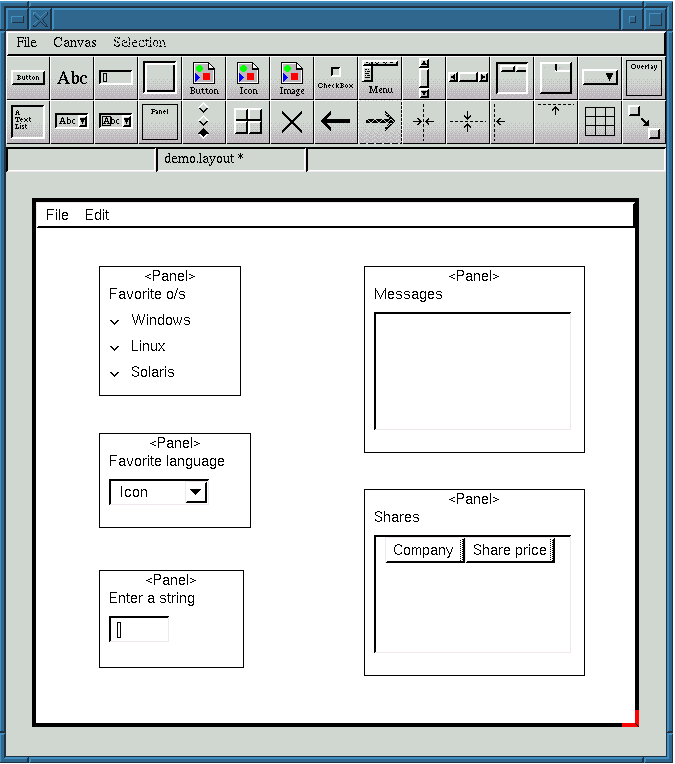
\includegraphics[width=4.0in,height=3.8in]{ub-img/ub-img60.png}
\end{center}

{\sffamily\bfseries Figure 18-11:}
{\sffamily Ivib main window}

To create a dialog window using Ivib, start the program with the name of
a new source file. For example:

\iconcode{
\>   \ \ ivib myprog.icn}

The Ivib window will appear with a blank
"canvas" area, which represents the dialog
window to be created. At startup, the attributes of this window are the
default Icon window attributes. Before you learn how to change these
attributes, here is how you add a button to the dialog. Clicking the
button in the top left-hand corner of the toolbar does this. Try moving
and resizing the resulting button by left-clicking on it with the
mouse. To change the label in the button, click on it so that the red
borders appear in the edges. Then press Alt-D. The dialog shown in
Figure 18-12 (left) appears.
Change the label by simply changing the text in the
"Label" field and clicking "Okay".

\bigskip

\noindent 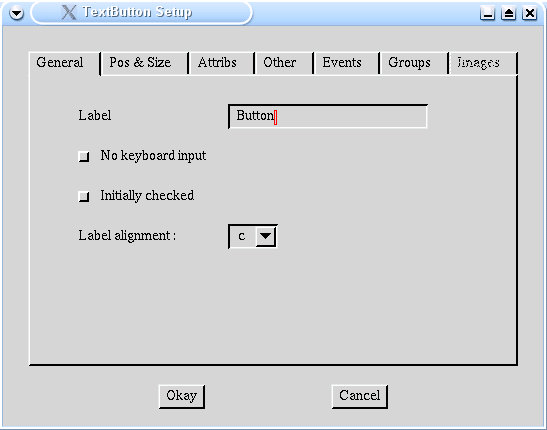
\includegraphics[width=3.125in,height=2.62in]{ub-img/ub-img61.jpg}
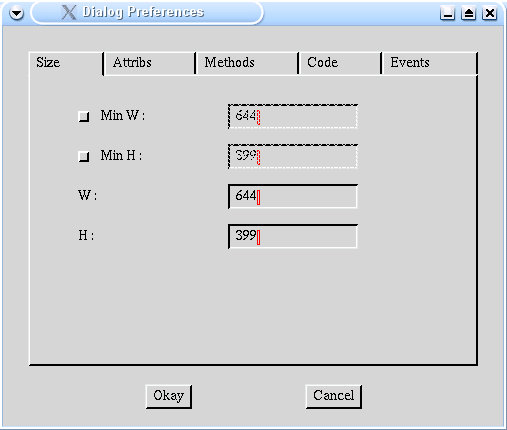
\includegraphics[width=3.125in,height=2.62in]{ub-img/ub-img63.jpg}

{\sffamily\bfseries Figure 18-12}
{\sffamily Button (left) and Dialog (right) configuration windows}

\bigskip

As just mentioned, the dialog's attributes are
initially the default window attributes. To change these, select the
menu option Canvas -{\textgreater} Dialog prefs. The window shown in
Figure 18-12 (right) appears. To change the dialog attributes:

\begin{enumerate}
\item \ Click on the Attribs tab

\item \ Click on the Add button


\item Edit the two text fields so that they hold the attribute name and
the attribute value respectively; for example try adding
"bg" and "pale blue".
\item \ Click on Apply.

\item Click on Okay.
\end{enumerate}

\bigskip

Note that the button changes its background to pale blue too. Each
object has its own attributes that it can set to override the dialog
attributes. Click on the button and press Alt-D to bring up the
button's configuration dialog again. Now click on the
Attribs tab of this dialog and set the background color to white, for
example. Then click okay and you will see that the
button's background changes to white.

You will recall from the previous example programs that some objects can
be contained in other objects, such as the \texttt{Panel} class. This
is handled conveniently in Ivib. Add a \texttt{Panel} object to the
dialog by clicking on the \texttt{Panel} button (on the second row,
fourth from the left). A panel appears. Now drag the button into the
panel. A message should appear in the information label below the
toolbar, "Placed inside container." Now try
dragging the panel about, and you will observe that the button moves
too - it is now "inside" the panel.
Dragging it outside the panel's area moves it back
out. This method applies to all the container objects.

There are several buttons that operate on objects. The large
"X" button deletes the currently selected
objects. Try selecting the button and deleting it. The arrow buttons
are "redo" and
"undo" operations. Clicking on the undo
button will undo the delete operation and the button should reappear.

Now try saving your canvas. Press Alt-S, and select a filename, or
accept the default. At the end of an ivib-enhanced Unicon source file
is a gigantic comment containing ivib's layout
information. This comment is \index{ASCII}ASCII text, but it is not
really human-readable. If the program is called, for example,
\texttt{myprog.icn}, then this can be compiled with

\iconcode{
\>   unicon myprog}

\noindent
to give an executable file \texttt{myprog} that, when run, will produce
the same dialog shown in the canvas area. Of course, the resulting
dialog will not do anything, and it is then up to the programmer to
fill in the blanks by editing \texttt{myprog.icn}.

Hopefully, following the above steps will give you an idea of how the
Ivib program works. Below are more details regarding the individual
components, dialogs, and operations.

\subsection*{Moving, selecting and resizing}

Select an object by clicking on it with the mouse. Its selection is
indicated by red edges around the corners. Multi-select objects by
holding the shift key down and clicking on the objects. The first
selected object will have red corners; the others will have black
corners. There are several functions which operate on multiple objects
and map some attribute of the first selected object to the others;
hence the distinction.

To move an object, select it by clicking on it with the left mouse
button, and then drag it. Note that dragging an object even by one
pixel will set the X or Y position to an absolute figure, disturbing
any carefully set up percentage specification! Because this can be
irritating when done accidentally, the X and/or Y position may be fixed
in the dialog so that it cannot be moved in that plane. Alternatively,
when selecting an object that you do not intend to move, use the right
mouse button instead.

To resize an object, select it and then click on one of the corners. The
mouse cursor will change to a resize cursor and the corner may be
dragged. Note that, like the position specification, resizing an object
will set the size to an absolute number and will also reset the
"use default" option. Again, this can be
avoided by fixing the width and/or height in the object's dialog box.

\subsection*{Dialog configuration}

This dialog, accessed via the menu selection \ \texttt{Canvas
-{\textgreater} Dialog prefs} allows the user to configure some general
attributes of the dialog being created. \ The tabs are described in
this section.

\paragraph{Size}
The minimum width and height entries simply set the minimum dimensions
of the window. The width and height may be configured here, or more
simply by resizing the canvas area by clicking on the red bottom
right-hand corner.

\paragraph{Attribs}
This has been described briefly above; the Add button produces a new
entry that is then edited. The edited entry is placed in the table with
Apply. The Delete button deletes the currently highlighted selection.

\paragraph{Code generation}
The part of the code to setup the dialog is written into a method called
setup. If the "interpose in existing file"
option is checked, then the program will read the present contents of
the selected output file up to the current setup method, interpose the
new setup, and copy the remainder out. This is useful if some changes
have been made to the file output by a previous run. It is
important to take a copy of the existing file before using this option,
in case unexpected results occur.

The other options simply select which other methods should be produced.
If a main procedure is produced, then the result will be an executable
program.

\paragraph{Other}
This tab allows the name of the dialog to be set, together with a flag
indicating whether it is "modal" or not. If
so, then a method called pending is produced. This method is repeatedly
called by the toolkit while it is waiting for events to occur.


\subsection*{Component configuration}

Each component dialog has a standard tabbed pane area for configuration
of attributes common to all components. The tabs are as follows:

\paragraph{Position \& size}
The X, Y, W and H options set the position and size of the object. The
drop-down list can be used for convenience, or a value may be entered
by hand. The "fix" buttons prevent the
object from being moved or sized outside the given parameter in the
Canvas area. This is useful once an object's position
has been finalized, and you don't wish to accidentally
move it. The "use default" buttons mean
that the width/height will be set as the default for the object based
on the parameters and the attributes. For example, a
button's size will be based on the label and the font.
For some objects there is no default size, so these buttons are shaded.
The alignment of the object is also set from this tab.

\paragraph{Attribs}
This works in exactly the same way as the Attribs tab for the dialog,
except that these attributes apply only to the object.

\paragraph{Other}
This tab allows the name used in the output program code to be set.
The "Draw
Border" button applies to some objects (see the reference
section in Appendix C for further information). If the
"Is Shaded" button is clicked, then the
initial state of the object will be shaded. If the "Has
initial focus" button is clicked, then this object will
have the initial \index{keyboard}keyboard focus when the dialog is
opened.

\subsection*{Component details}

Components are added to the dialog by clicking on the toolbar buttons,
and dialogs are produced by selecting the object and pressing Alt-D, as
explained above. Most of the dialogs are hopefully straightforward, but
some warrant further explanation.

\paragraph{TextButton}
The dialog for this component includes an option for the button to be
added to a \texttt{ButtonGroup} structure. This is explained in detail
shortly.

\paragraph{Border}
To select this component, rather than
clicking inside the border, click in the area at the bottom right hand
corner. It can then be resized or moved. Now try dragging another
object, such as a \texttt{CheckBox} or \texttt{Label} and release it so
that its top left-hand corner is within the area in the bottom
right-hand corner of the \texttt{Border} object. The
\texttt{CheckBox}/\texttt{Label} or whatever is now the title of the
\texttt{Border}. Thus, any object can be in the title. To remove the
object from the \texttt{Border}, just drag it out. The alignment of the
title object is set in the dialog, but is by default left aligned.

\paragraph{Image}
Initially the Image object has an outline. When a filename is entered
into the dialog however, the image itself is displayed.

\paragraph{CheckBox}
Customized up/down images may be set from the dialog, and a
\texttt{CheckBoxGroup} may be selected if one is available; this is
explained in more detail shortly.

\paragraph{MenuBar}
This dialog enables a complete multi-level menu to be
created. Clicking on a line allows an item to be inserted at that
point. Only menus can be inserted into the lowest level.
Clicking on an item will allow insertion, deletion, or editing of the
particular item. A \texttt{CheckBoxGroup} can be created by selecting
multiple check boxes (by holding down the Shift key while clicking on
the lines) and clicking the button.

\paragraph{ScrollBar}
Both vertical and horizontal scroll bars are available; for details of
how the various options work, please see the \index{reference}reference
manual for the toolkit.

\paragraph{Table}
A table column is added by clicking the Add button; the details should
then be edited and the Apply button pressed to transfer the details to
the table. A selected column can be deleted with the Delete button. The
drop-down list selects whether or not lines in the table can be
selected by clicking them.

\paragraph[TabSet]{TabSet}
Add a \texttt{TabItem} (a tabbed pane) by clicking the Add button.
A single pane is automatically present when the object is created.
To switch between panes, select a \texttt{TabItem} button. An asterisk
appears by the entry. When the dialog exits, this
\texttt{TabItem} is on the front of the \texttt{TabSet}. To add
items to the current pane, drag and drop them into it. The whole
of the item must be in the pane, and a confirmation message appears to
indicate that the item has been added to the container. To take it out
of the container, drag it out of the pane. Note that the selected
pane is the one that is configured to be initially at the front when
the dialog is opened.

\paragraph{MenuButton}
The \texttt{MenuButton} component is a menu system with one root
menu. The dialog is the same as \texttt{MenuBar}'s except that
the small icon can be configured.

\paragraph{OverlaySet}
The configuration for an \texttt{OverlaySet} is very similar to that for
a \texttt{TabSet}, except that there are no tab labels to configure of
course.

\paragraph{CheckBoxGroup}
This does not create an object, it
places several selected \texttt{CheckBox} objects into a
\texttt{CheckBoxGroup} object. They act as coordinated radio
buttons. To use this button, select several \texttt{CheckBox}
objects, and press the button.

The \texttt{CheckBoxGroup} is configured by selecting the menu
item Canvas -{\textgreater} CheckBoxes. The only attribute to
be configured is the name of the \texttt{CheckBoxGroup}. Once
a \texttt{CheckBoxGroup} has been created, it cannot be deleted. A
\texttt{CheckBox} can be taken out or put into a \texttt{CheckBoxGroup}
from its configuration dialog.

\paragraph{ButtonGroup}
The \texttt{ButtonGroup} operates in a very similar fashion to
\texttt{CheckBoxGroup}, except that it places buttons into a
\texttt{ButtonGroup}.



\subsection*{Other editing functions}

Other editing functions can be applied to
the dialog being created. They are accessed either via the toolbar,
the Selection menu, or the Edit menu.

\paragraph{Delete}
The Delete function simply deletes all the selected objects; note that
deleting a container also deletes all the objects inside it.

\paragraph{Undo and Redo}
The Undo and Redo functions undo and redo changes. The size of the
buffer used for storing undo information can be configured in the File
-{\textgreater} Preferences dialog; by default it allows 7 steps
backward at any one time.

\paragraph[Center Horizontally]{Center Horizontally}
The Center Horizontally operation sets the selected
objects' X position specification to
"50\%", their alignment to center, and
fixes them in that horizontal position. To
"unfix" an object, uncheck the
"fix" box in its dialog box. Center
vertically naturally works in just the same way for the y position.

\paragraph{Align Horizontally}
This operation sets the X position and alignment
of all the selected objects to the X position and alignment of
the first selected object. Whether the objects end up appearing to be
left-, center-, or right-aligned will depend on the alignment of the
first selected object. "Align vertically"
works just the same way.

\paragraph{Grid}
To use the Grid function, place several items roughly in a grid, select
them all, perform the operation, and hopefully they will be nicely
aligned.

\paragraph{Copy}
The Copy function simply creates a duplicate of each selected object.

\paragraph{Equalize widths}
This function simply copies the width of the first
selected object to all of the other selections. "Equalize
heights" naturally does the same for heights.

\paragraph{Even Space Horizontally}
This operation moves the objects so that they are
equally spaced between the leftmost and rightmost objects of the
current selections, which are not moved. "Even Space
Vertically" does the same vertically.

\paragraph{Reorder}
The Reorder function is used to reorder the selected objects in the
program's internal lists. This is useful so that they
are produced in the program output in the desired order, for example to
ensure that the tab key moves from object to object in the right
sequence. By selecting several objects and using reorder, those objects
appear first in sequence in the order in which they were selected.

\section{Summary}

The Unicon GUI toolkit offers a full-featured, attractive way of
constructing interfaces. The toolkit has many features--tables,
tabbed property sheets, and multi-line text editing capability--that
are not present in Icon's vidgets GUI
library. Many components present in both libraries are more
flexible in the GUI toolkit, supporting fonts, colors, and graphics
that the vidgets library does not handle. The ivib interface
builder tool provides programmers with easy access to the GUI toolkit.

Object-orientation mainly affects this class library's
extensibility, although it also contributes to the
simplicity of the design. Inheritance, including multiple inheritance,
is used extensively in the 37 classes of the GUI toolkit. Inheritance
is the main object-oriented feature that could not be easily mimicked
in a procedural toolkit such as the vidgets library, and inheritance is
the primary extension mechanism.
